% Autor: Leonhard Segger, Alexander Neuwirth
% Datum: 2017-10-30
\documentclass[
	% Papierformat
	a4paper,
	% Schriftgröße (beliebige Größen mit „fontsize=Xpt“)
	12pt,
	% Schreibt die Papiergröße korrekt ins Ausgabedokument
	pagesize,
	% Sprache für z.B. Babel
	ngerman
]{scrartcl}

% Achtung: Die Reihenfolge der Pakete kann (leider) wichtig sein!
% Insbesondere sollten (so wie hier) babel, fontenc und inputenc (in dieser
% Reihenfolge) als Erstes und hyperref und cleveref (Reihenfolge auch hier
% beachten) als Letztes geladen werden!

% Silbentrennung etc.; Sprache wird durch Option bei \documentclass festgelegt
\usepackage{babel}
% Verwendung der Zeichentabelle T1 (Sonderzeichen etc.)
\usepackage[T1]{fontenc}
% Legt die Zeichenkodierung der Eingabedatei fest, z.B. UTF-8
\usepackage[utf8]{inputenc}
% Schriftart
\usepackage{lmodern}
% Zusätzliche Sonderzeichen
\usepackage{textcomp}

% Mathepaket (intlimits: Grenzen über/unter Integralzeichen)
\usepackage[intlimits]{amsmath}
% Ermöglicht die Nutzung von \SI{Zahl}{Einheit} u.a.
\usepackage{siunitx}
% Zum flexiblen Einbinden von Grafiken (\includegraphics)
\usepackage{graphicx}
% Abbildungen im Fließtext
\usepackage{wrapfig}
% Abbildungen nebeneinander (subfigure, subtable)
\usepackage{subcaption}
% Funktionen für Anführungszeichen
\usepackage{csquotes}
% Zitieren, Bibliographie
\usepackage{biblatex}


% Zur Darstellung von Webadressen
\usepackage{url}
%chemische Formeln
\usepackage[version=4]{mhchem}
% siunitx: Deutsche Ausgabe, Messfehler getrennt mit ± ausgeben
\usepackage{floatrow}
\floatsetup[table]{capposition=top}
% Verlinkt Textstellen im PDF-Dokument
\usepackage[unicode]{hyperref}
% "Schlaue" Referenzen (nach hyperref laden!)
\usepackage{cleveref}
\sisetup{
	locale=DE,
	separate-uncertainty
}
%\bibliography{6Mi_M3_29-11-2017_References}

\begin{document}
	
	\begin{titlepage}
		\centering
		{\scshape\LARGE Versuchsbericht zu \par}
		\vspace{1cm}
		{\scshape\huge E1 - Gleich- und Wechselstrom\par}
		\vspace{2.5cm}
		{\LARGE Gruppe 6Mi \par}
		\vspace{0.5cm}
		
		{\large Alexander Neuwirth (E-Mail: a\_neuw01@wwu.de) \par}
		{\large Leonhard Segger (E-Mail: l\_segg03@uni-muenster.de) \par}
		\vfill
		
		durchgeführt am 20.12.2017\par 
		betreut von\par
		{\large Philipp Eickholt} %Anpassen war das Fabian Schöttke? Nein    im Laborbuch steht nichts                         
		
		\vfill
		
		{\large \today\par}
	\end{titlepage}
	\tableofcontents
	\newpage


	\section{Kurzfassung}
	%TODO Hypothese	und deren Ergebnis
	%TODO Ergebnisse, auch Zahlen, mindestens wenn's halbwegs Sinn ergibt
	%TODO Was wurde gemacht
	
	\section{Methoden}
	%TODO Bilder von der Website klauen
	
	\section{Ergebnisse und Diskussion}
	%TODO Datenanalyse -> Überschrift?
	%TODO Unsicherheiten
	%TODO Spannungs messung ohne Strom fluss wurde Widerstan auf 2000 Ohm geschätz -> Satz
	In \cref{Spannung1} ist die Klemmspannung gegen den Strom, der sich aus $I = U/R$ ergeben hat, aufgetragen. 
	Es wurde ein linearer Fit durchgeführt, da nach der Theorie ein linearer Zusammenhang besteht. 
	Die Steigung der Geraden ist der (negative) Innenwiderstand $R_\text{i} = \SI{27,19 \pm 0,47}{\Omega}$.

	Trägt man die Leistung gegen den Außenwiderstand, ist zuerwarten, dass (genau) ein Maximum bei $R_\text{i}  R_\text{a}$ liegt.
	\cref{Leistung1} stellt dies und einen Fit mit dem \enquote{Scaled Levenberg-Marquardt}-Algorithmus, welcher die Methode der kleinsten Quadrate verwendet, dar. 
	Die Funktion des Fits ist:
	\begin{equation}
		f(x)=a\frac{x}{(x+b)^2}
	\end{equation}
	Es ergibt sich ein Parameter $b = \SI{29,51}{}$ ohne Unsicherheit, desshalb haben wir diese als relative Unsicherheit mit 2\% abgeschätzt. 
	Folglich ist $R_\text{i} = \SI{29,51 \pm 0,59}{\Omega}$.

	Analog kann man aus \crefrange{Spannung3Reihe}{Leistung3Parallel} die Innenwiderstände für drei parallel, bzw. in Reihe, geschaltete Akkus erhalten.
	In \cref{Tabelle_Innenwiderstaende} sind die ermittelten Innenwiderstände aufgelistet. 
	Aus diesen Widerständen lässt der Innenwiderstand eines einzelnen Akkus bestimmen.
	\cref{Tabelle_Innenwiderstaende2} zeigt diese. %TODO ihhhhh zeigt
	\begin{table}[tb]
		\centering
		\begin{tabular}{ r | c | c | c}
			Innenwiderstand& Ein Akku & 3 Akkus Reihe & 3 Akkus Parallel \\ \hline
			aus Klemmspannung& \SI{27,19 \pm 0,47 }{\Omega}& \SI{81,24 \pm 1,06 }{\Omega}&  \SI{9,73 \pm 0,20 }{\Omega} \\
			aus Leistung & \SI{29,51 \pm 0,59 }{\Omega}&  \SI{77,53 \pm 1,55 }{\Omega}&  \SI{9,79 \pm 0,19 }{\Omega}\\

		\end{tabular}
		\caption{Gemessener Innenwiderstand.}
		\label{Tabelle_Innenwiderstaende} 
	\end{table}
	\begin{table}[tb]
		\centering
		\begin{tabular}{ r | c | c | c}
			Innenwiderstand& Ein Akku & Akku Reihe & Akku Parallel \\ \hline
			aus Klemmspannung& \SI{27,19 \pm 0,47 }{\Omega}& \SI{27,08 \pm 0,35 }{\Omega}&  \SI{29,19 \pm 0,60 }{\Omega} \\
			aus Leistung & \SI{29,51 \pm 0,59 }{\Omega}&  \SI{25,84 \pm 0,52 }{\Omega}&  \SI{29,37 \pm 0,57 }{\Omega}\\

		\end{tabular}
		\caption{Gemessener Innenwiderstand.}
		\label{Tabelle_Innenwiderstaende2} 
	\end{table}

	\begin{figure}[tb]
		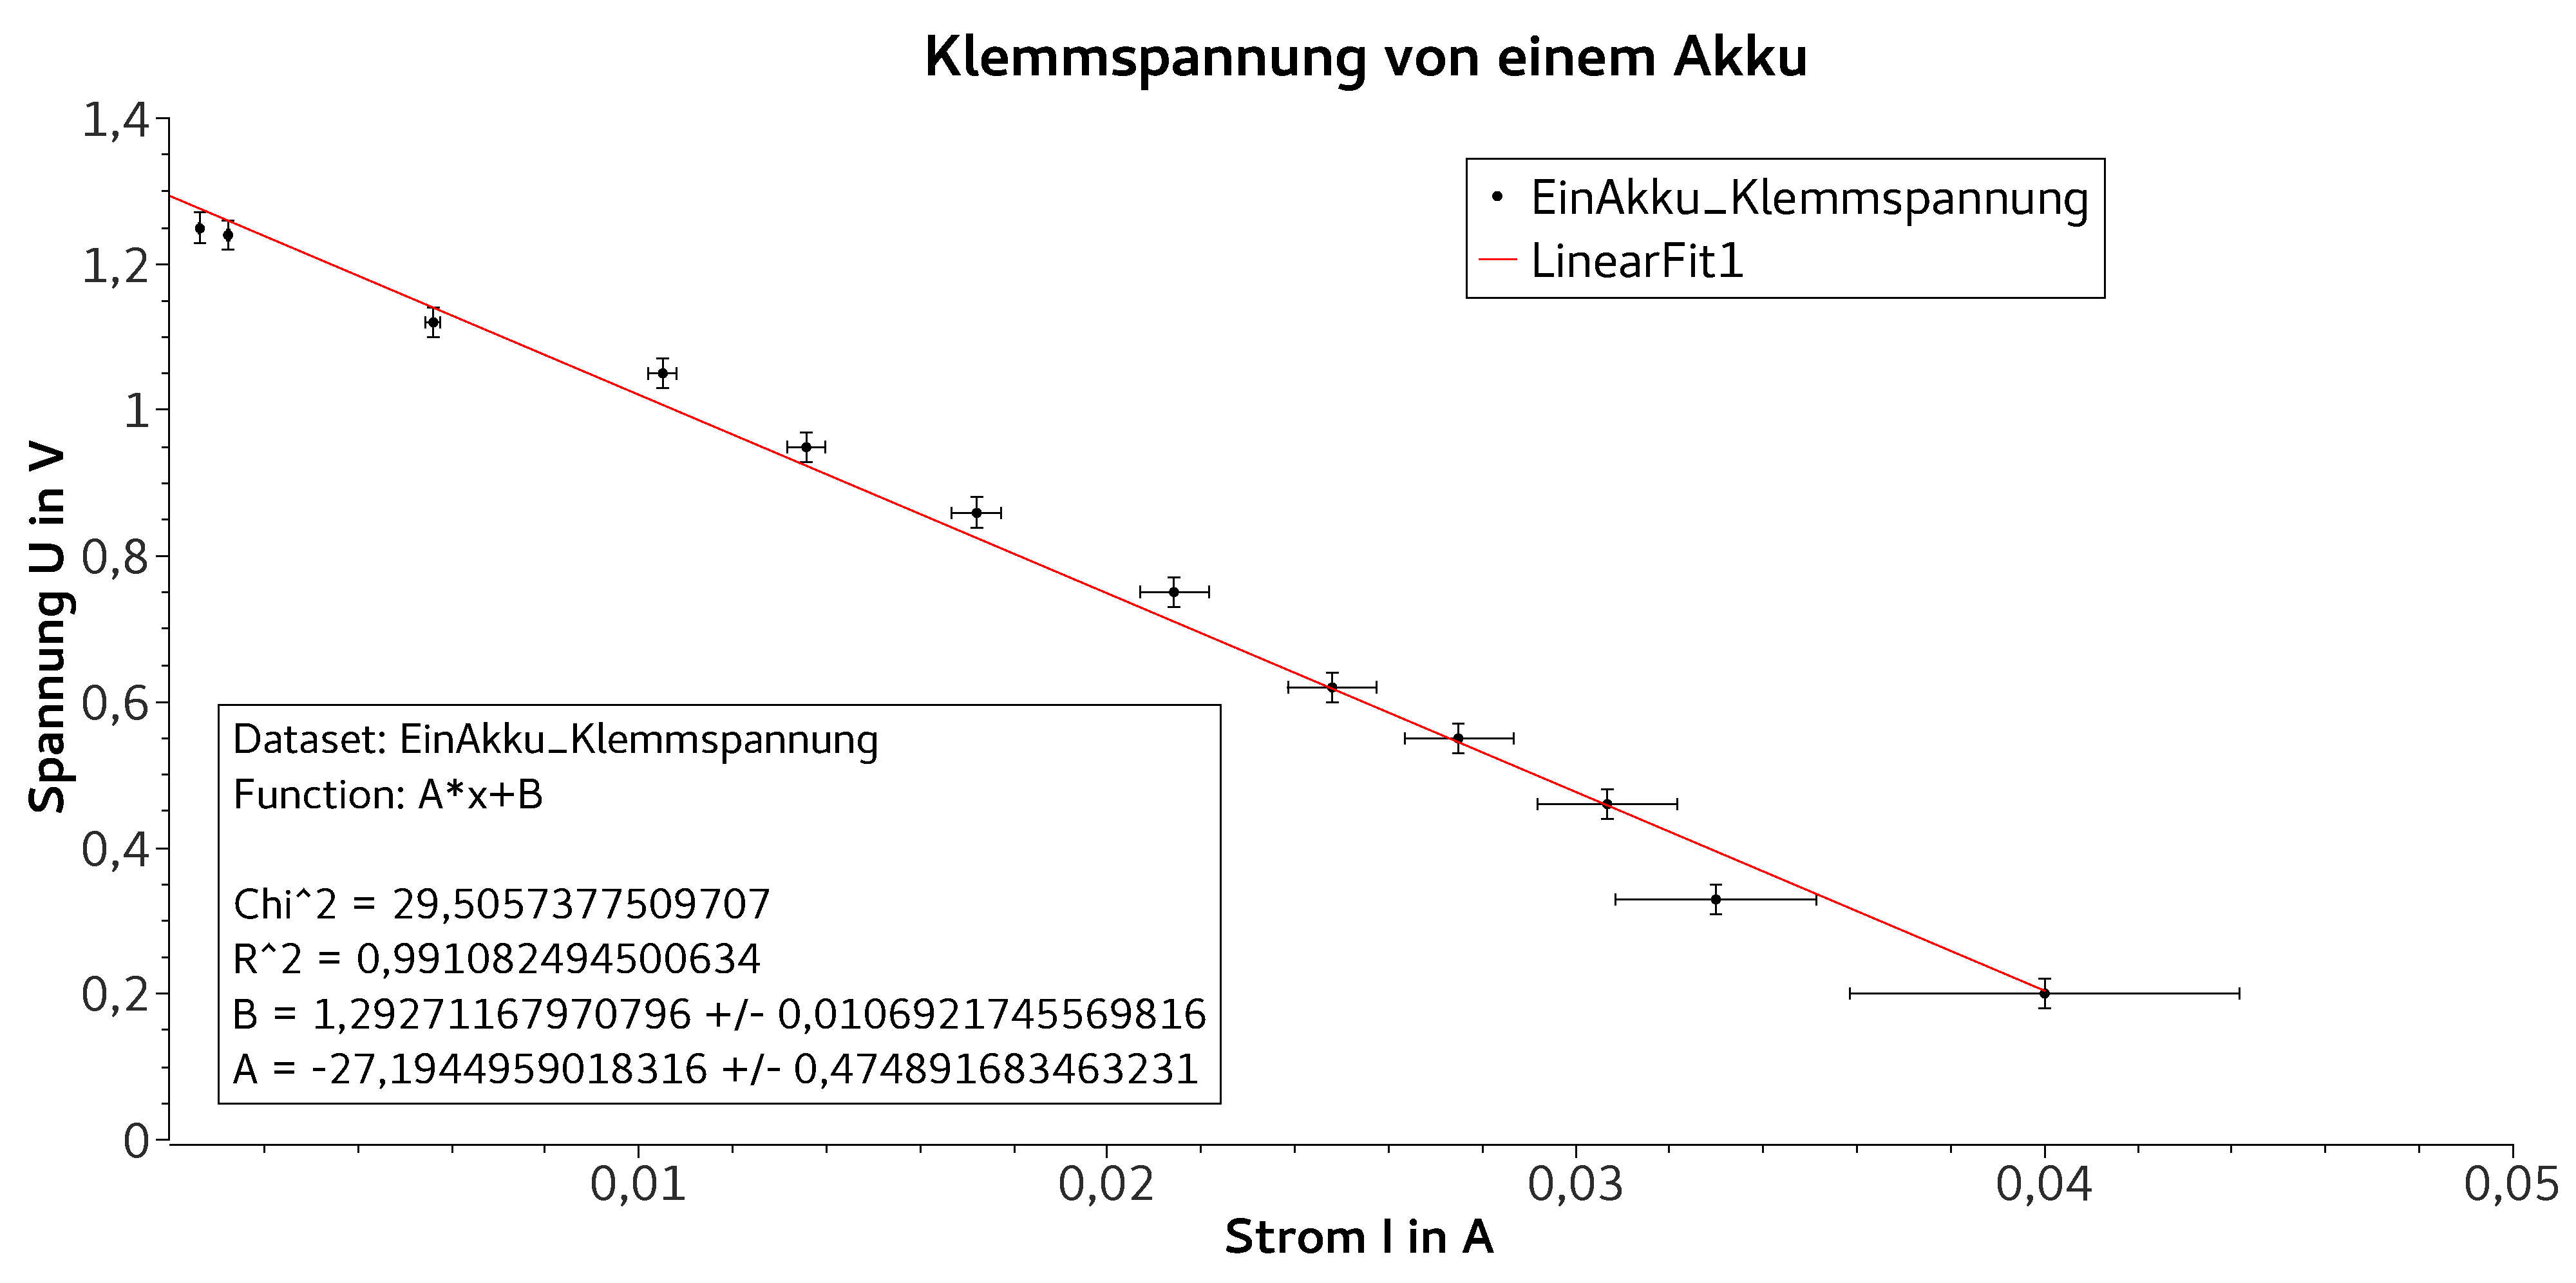
\includegraphics[width=1\textwidth]{Spannung1}
		\centering
		\caption{Die gemessene Klemmspannung bei einem Akku ist gegen den Strom aufgetragen.}
		\label{Spannung1}
		\centering
	\end{figure} 
	\begin{figure}[tb]
		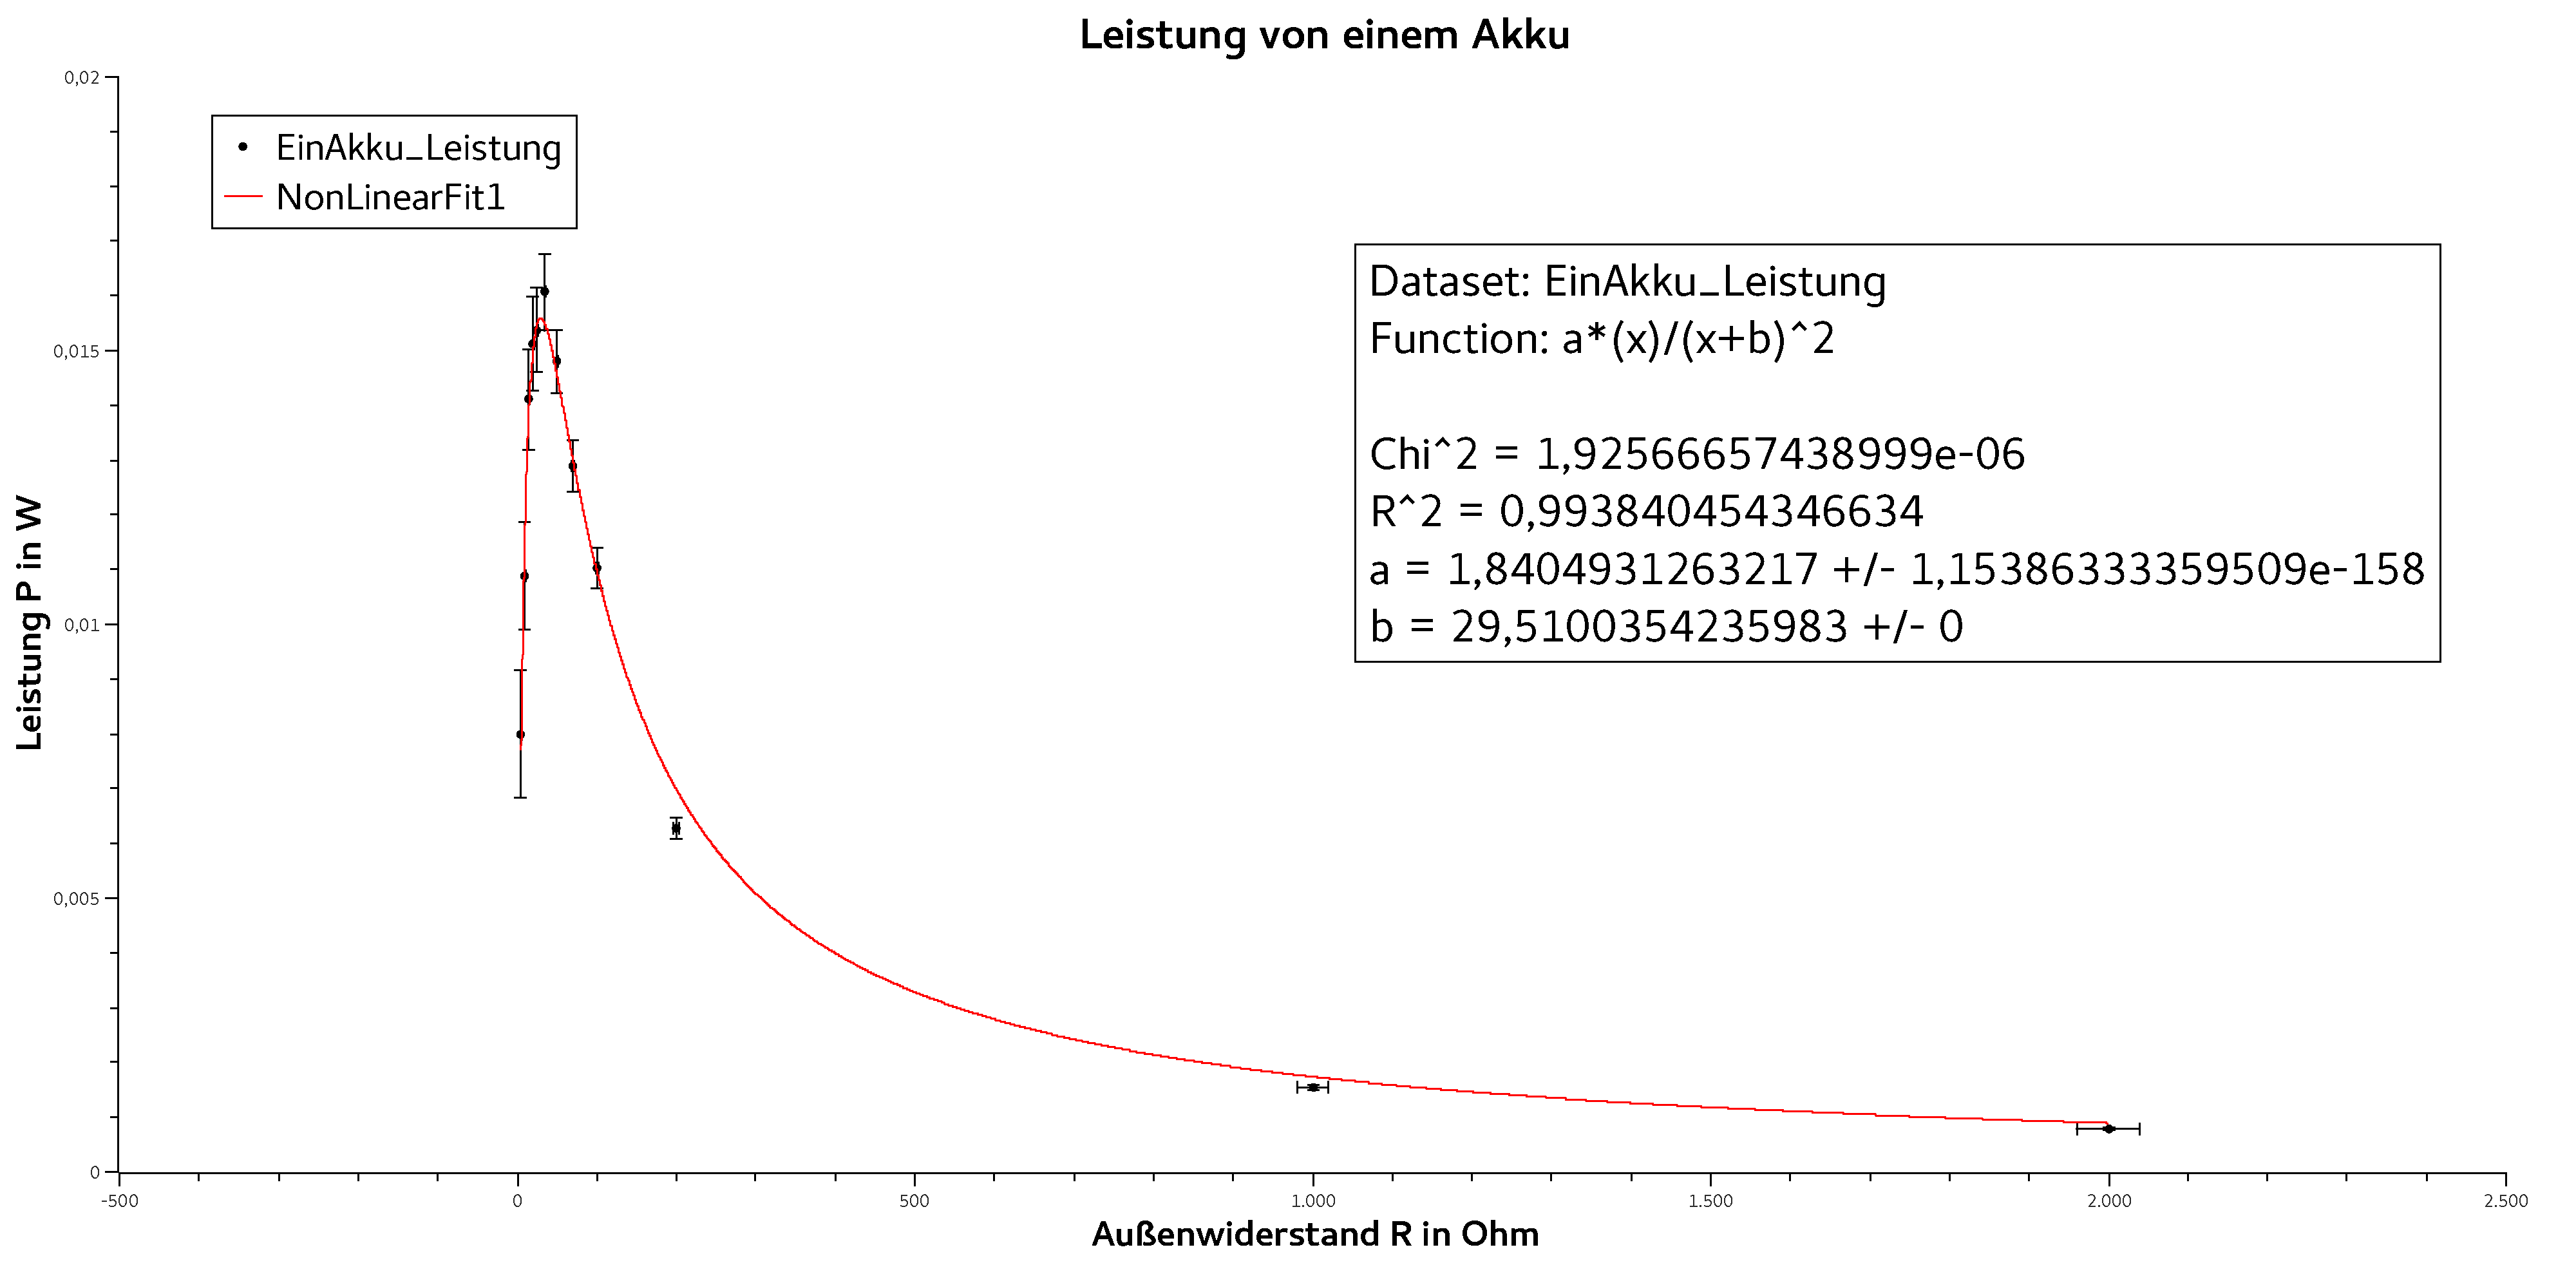
\includegraphics[width=1\textwidth]{Leistung1}
		\centering
		\caption{Die gemessene Leistung bei einem Akku ist gegen den Außenwiderstand aufgetragen.}
		\label{Leistung1}
		\centering
	\end{figure}
	\begin{figure}[tb]
		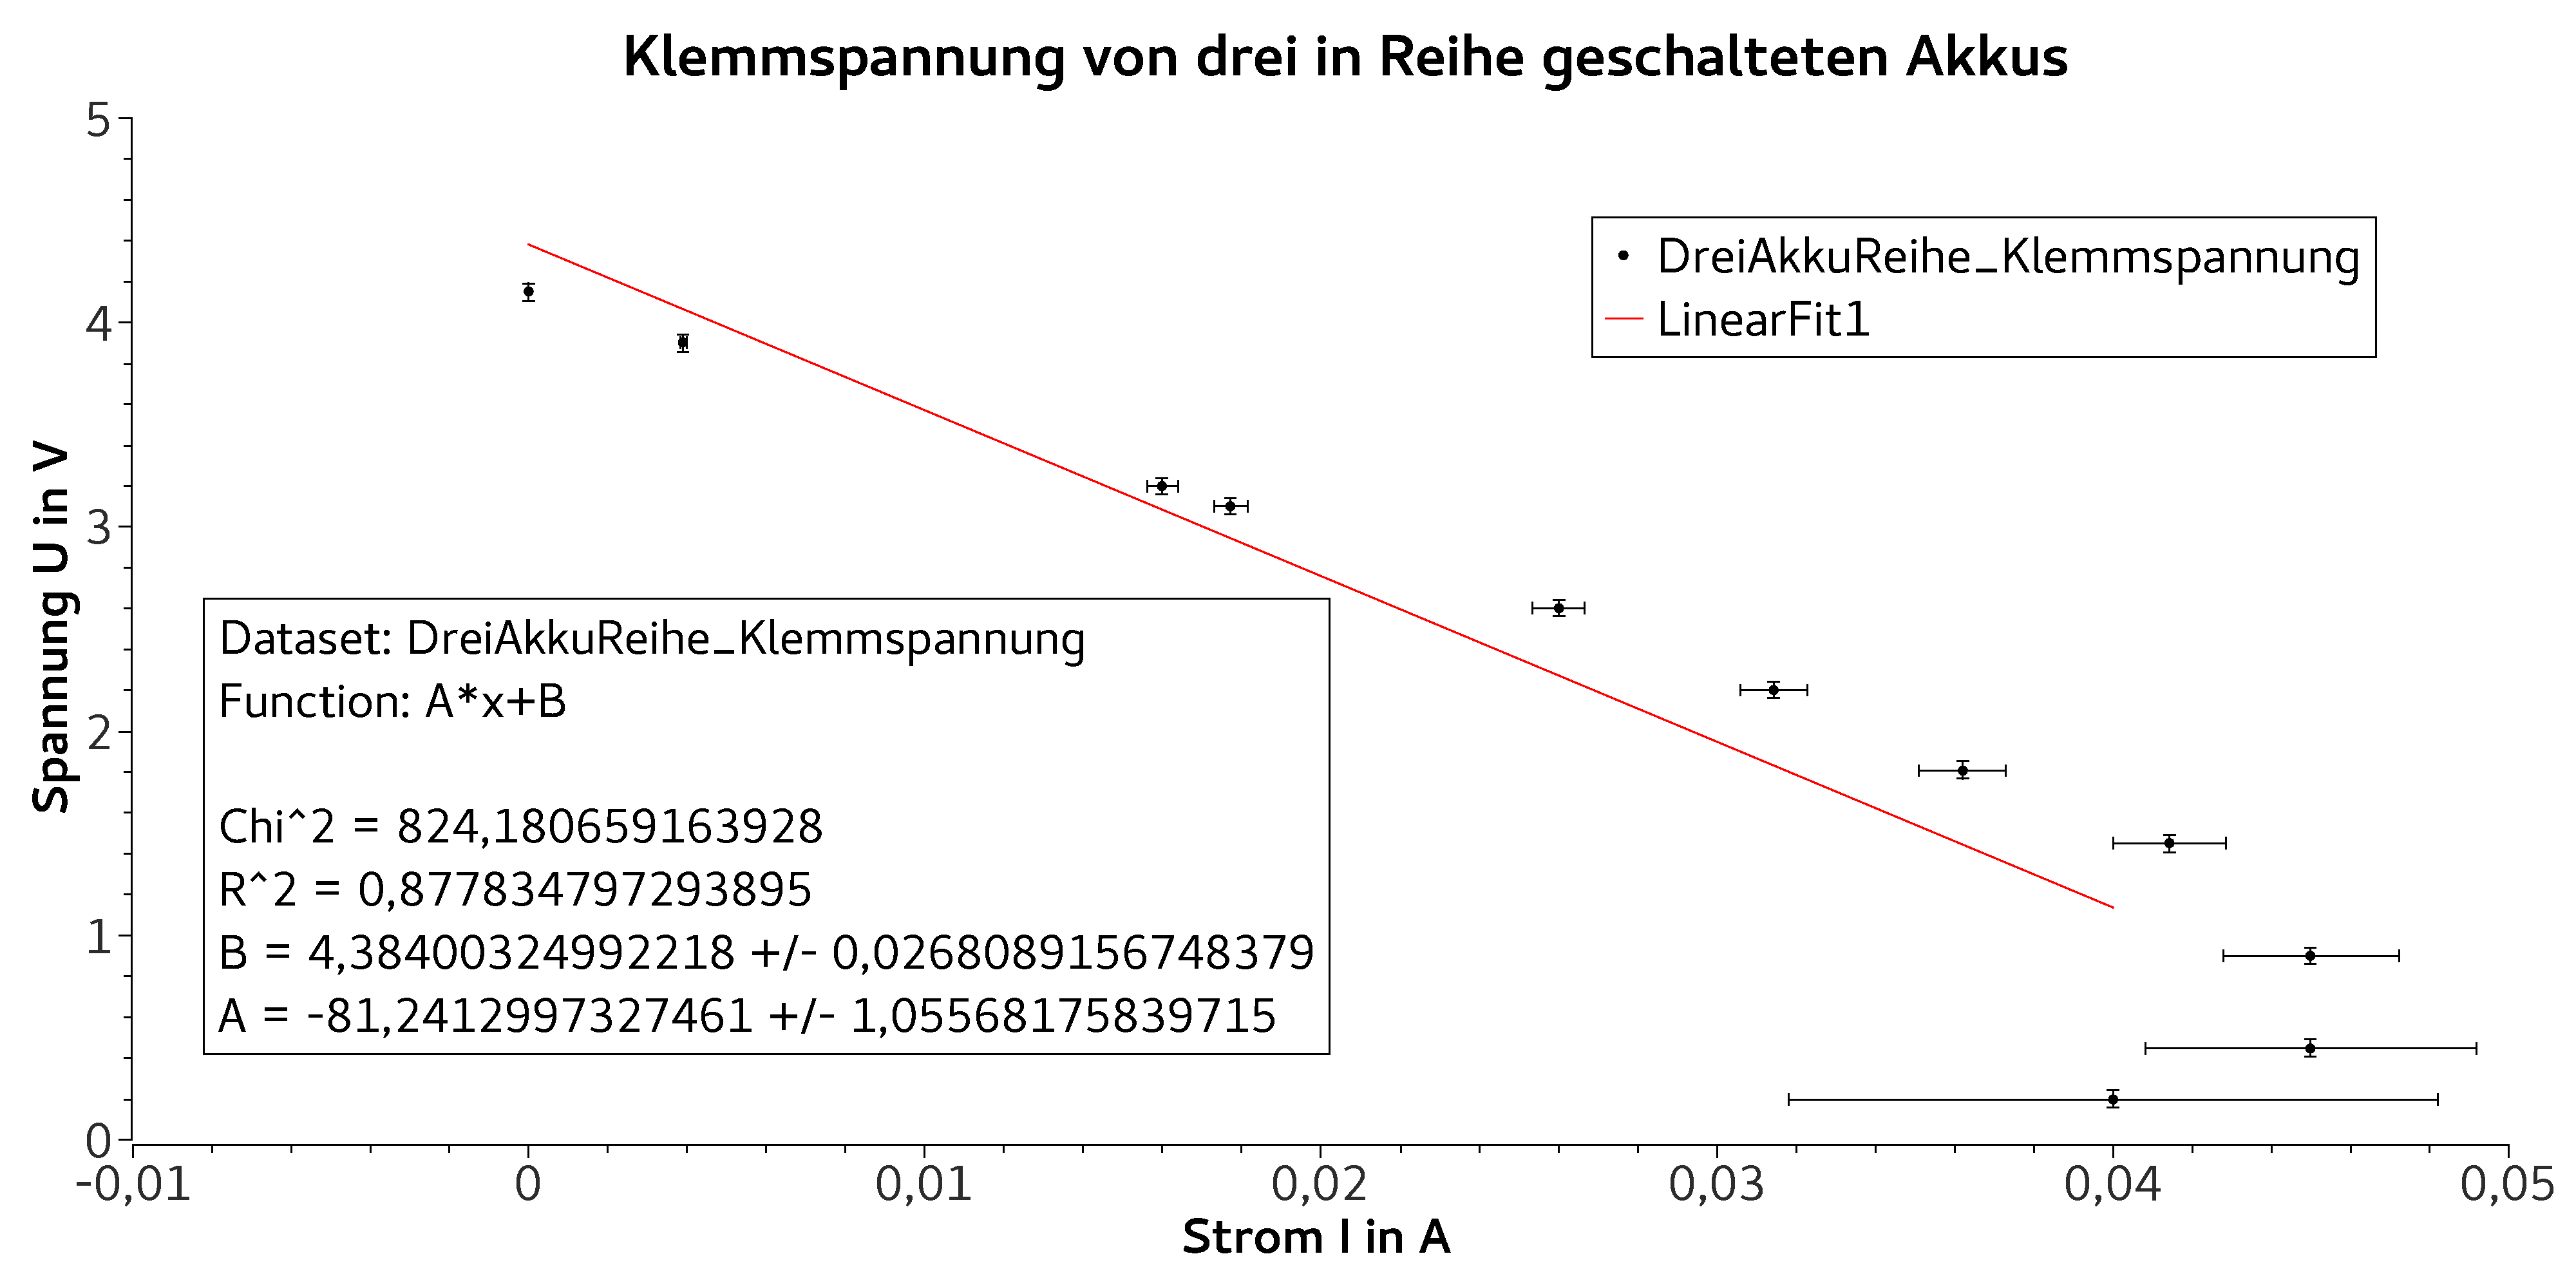
\includegraphics[width=1\textwidth]{Spannung3Reihe}
		\centering
		\caption{Die gemessene Klemmspannung bei drei in Reihe geschateten Akkus ist gegen den Strom aufgetragen.}
		\label{Spannung3Reihe}
		\centering
	\end{figure} 
	\begin{figure}[tb]
		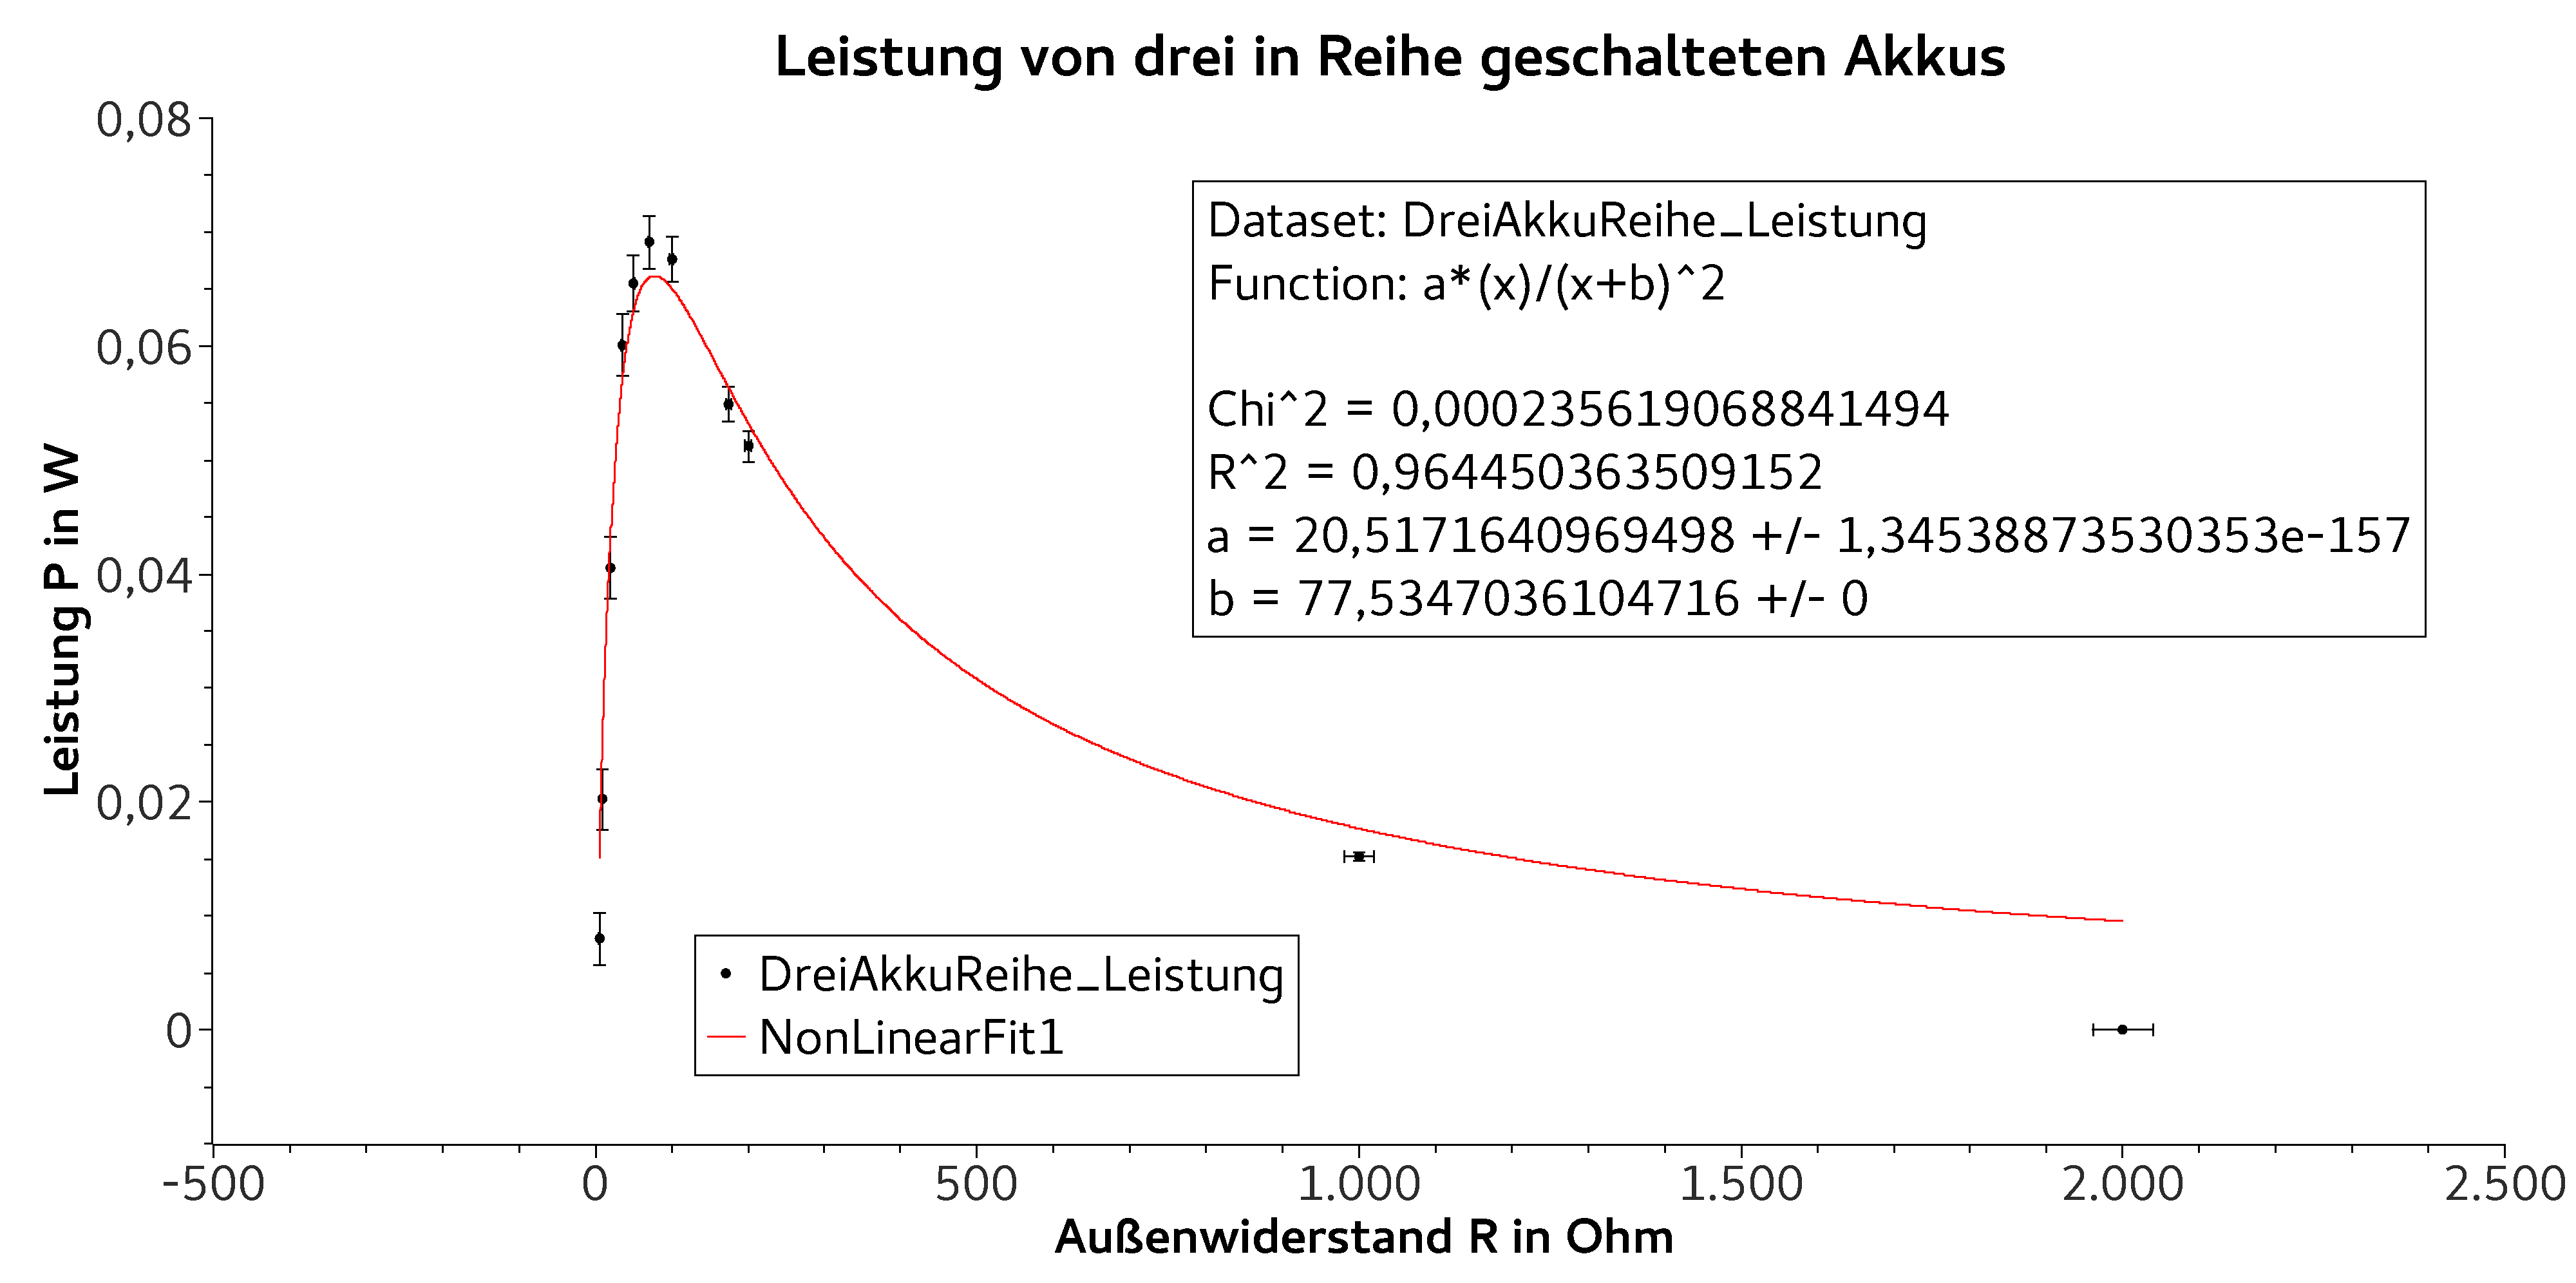
\includegraphics[width=1\textwidth]{Leistung3Reihe}
		\centering
		\caption{Die gemessene Leistung bei drei in Reie geschalteten Akkus ist gegen den Außenwiderstand aufgetragen.}
		\label{Leistung3Reihe}
		\centering
	\end{figure}
	
	\begin{figure}[tb]
		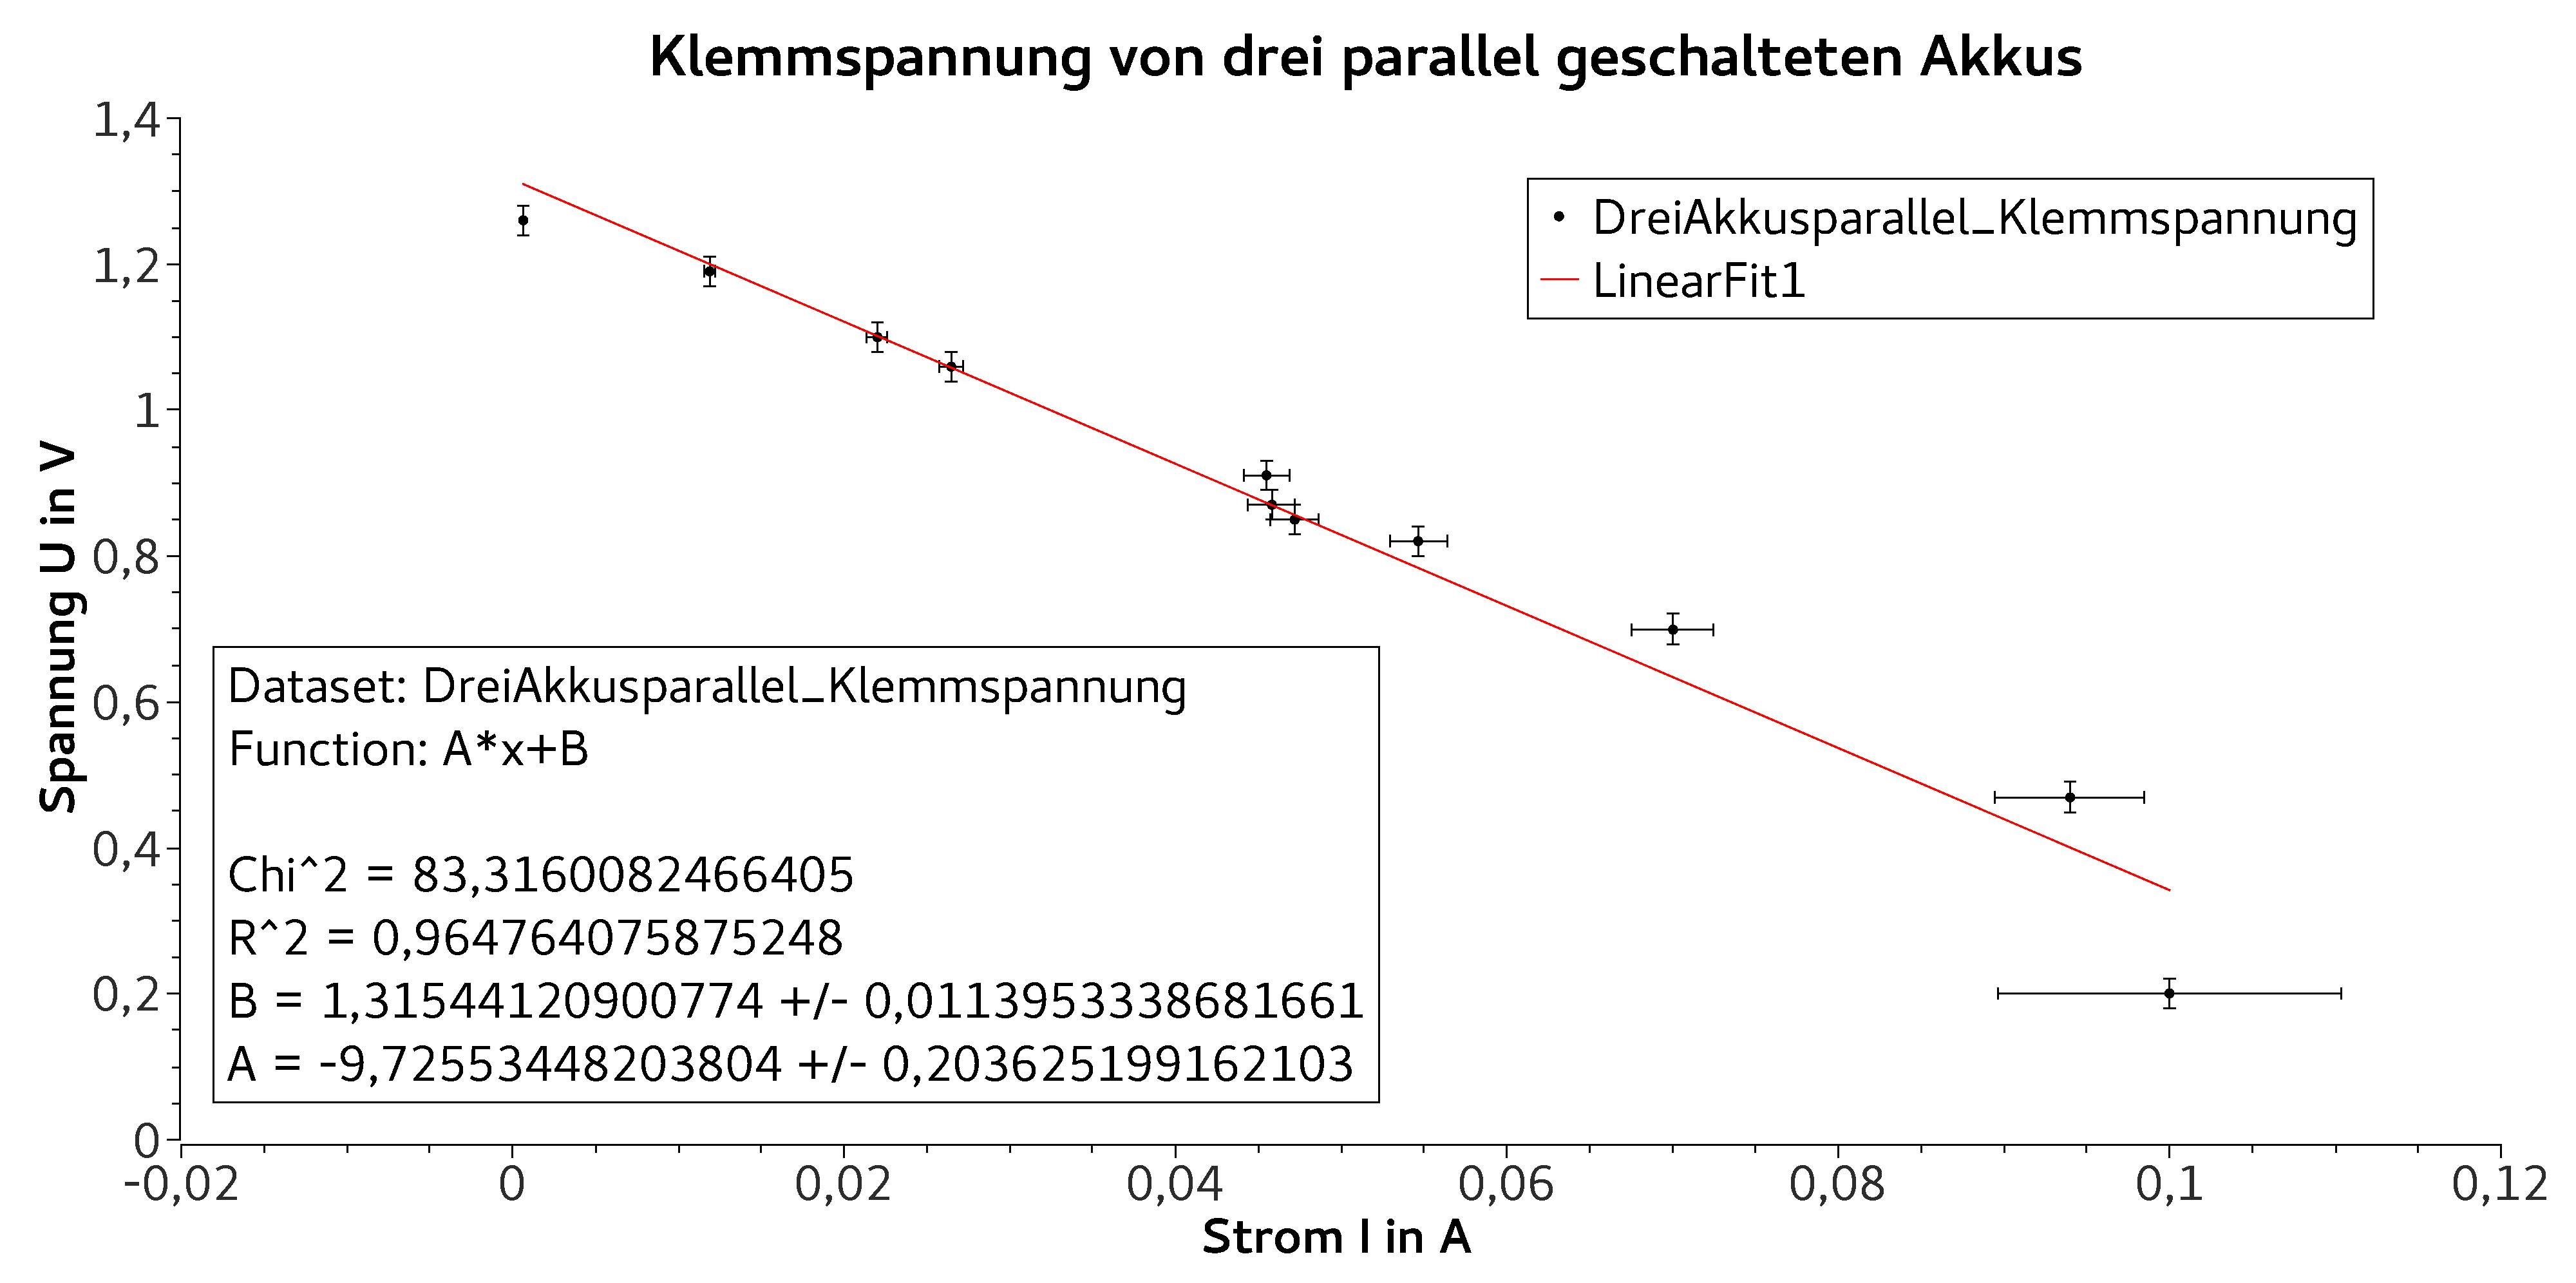
\includegraphics[width=1\textwidth]{Spannung3Parallel}
		\centering
		\caption{Die gemessene Klemmspannung bei 3 parallelen Akkus ist gegen den Strom aufgetragen.}
		\label{Spannung3Parallel}
		\centering
	\end{figure}

	\begin{figure}[tb]
		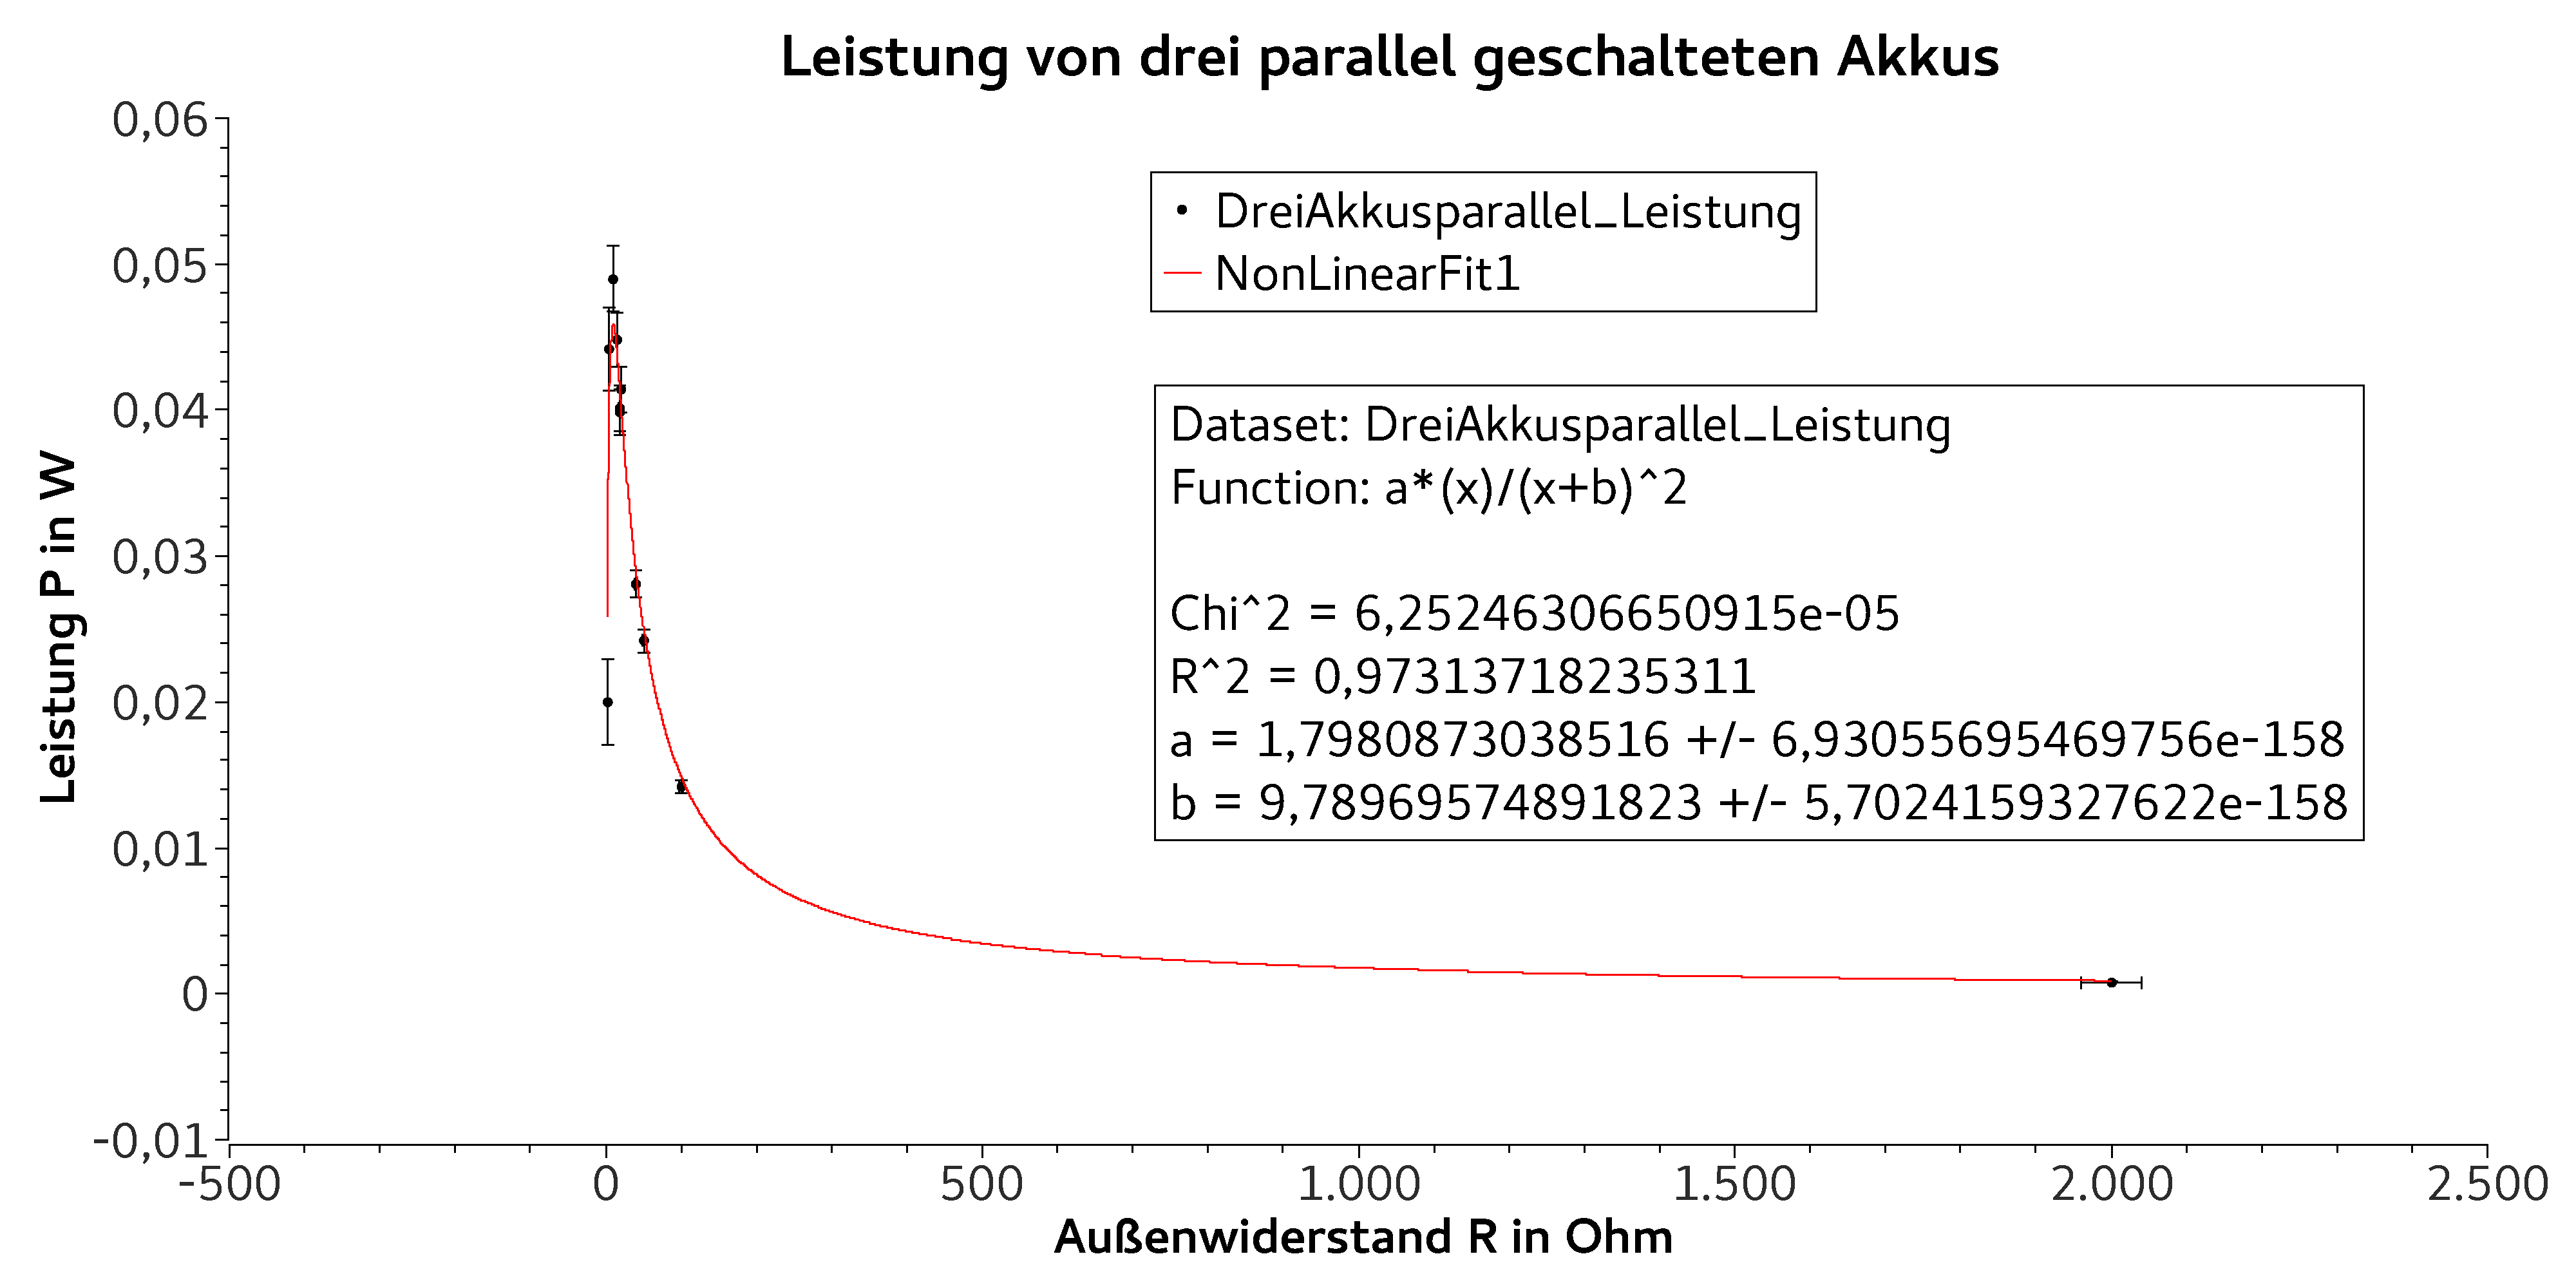
\includegraphics[width=1\textwidth]{Leistung3Parallel}
		\centering
		\caption{Die gemessene Leistung bei drei parallelen Akkus ist gegen den Außenwiderstand aufgetragen.}
		\label{Leistung3Parallel}
		\centering
	\end{figure}
	%TODO Zusatzfrage beantworten => Für das eine viele Parallel fürs andere in Reihe
	%TODO differenzieren zwischen wechsel und gleich in den Graph Beschreibungen
	\begin{figure}[tb]
		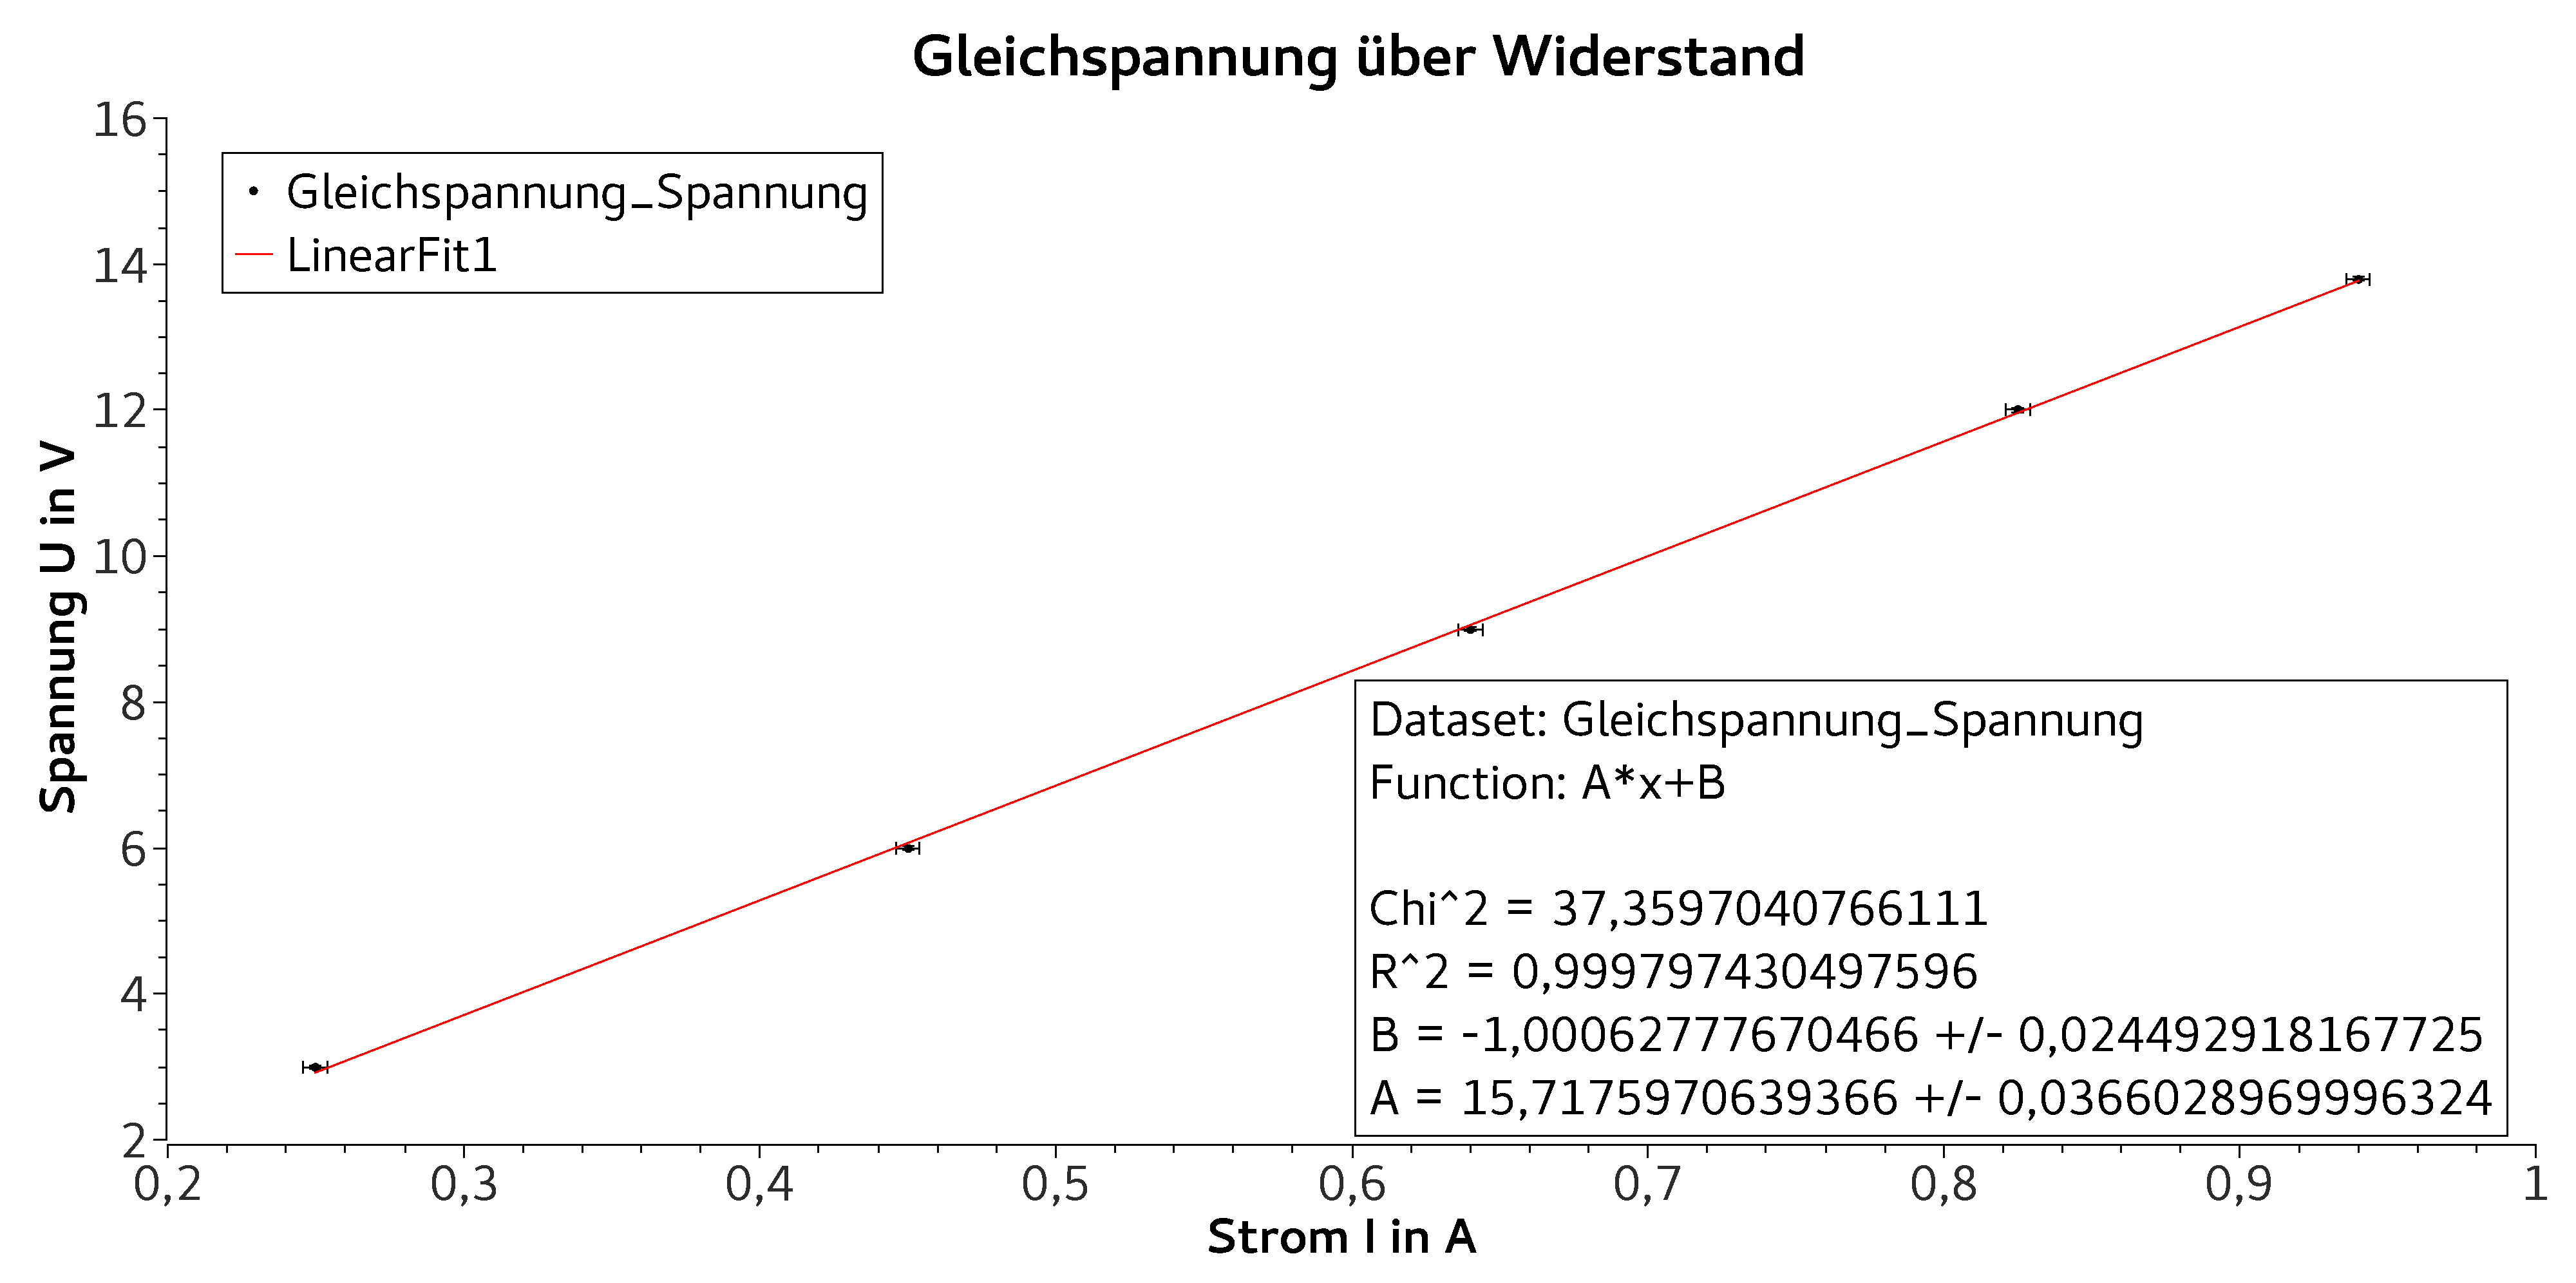
\includegraphics[width=1\textwidth]{WiderSpannungGleich}
		\centering
		\caption{Die gemessene Spannung ist gegen den Strom aufgetragen.}
		\label{WiderSpannungGleich}
		\centering
	\end{figure}
	\begin{figure}[tb]
		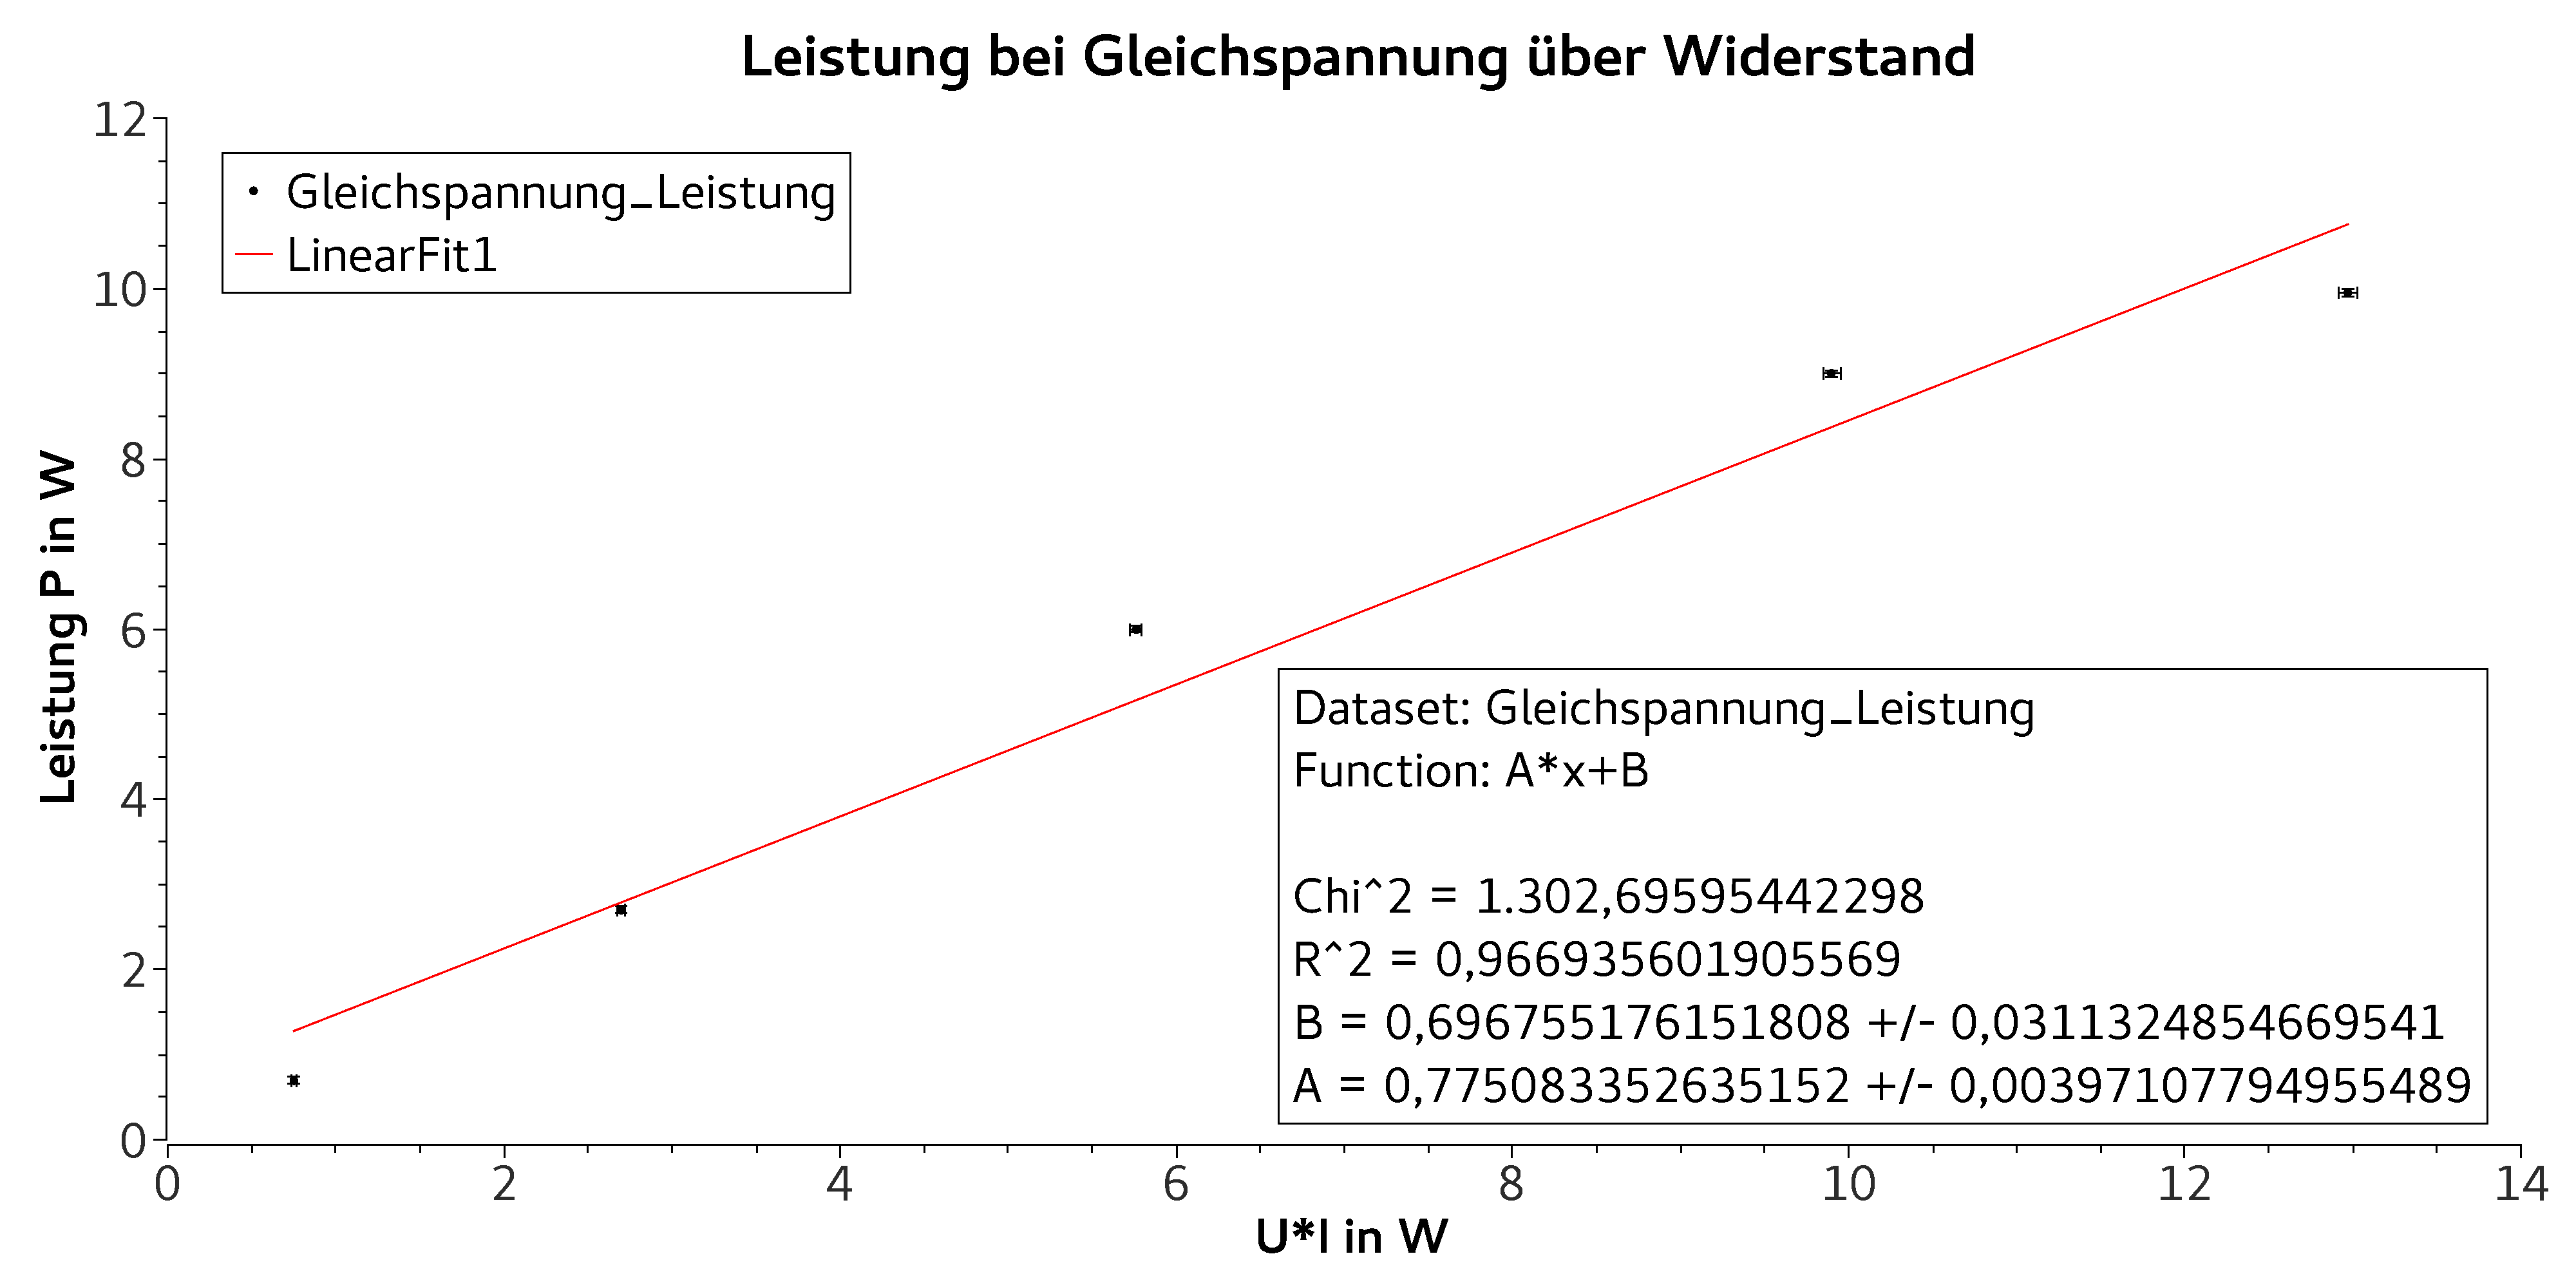
\includegraphics[width=1\textwidth]{WiderLeistungGleich}
		\centering
		\caption{Die gemessene Leistung ist gegen das Produkt aus Strom und Spannung aufgetragen.} %TODO ist des effektiv oder net?
		\label{WiderLeistungGleich}
		\centering
	\end{figure}
	\begin{figure}[tb]
		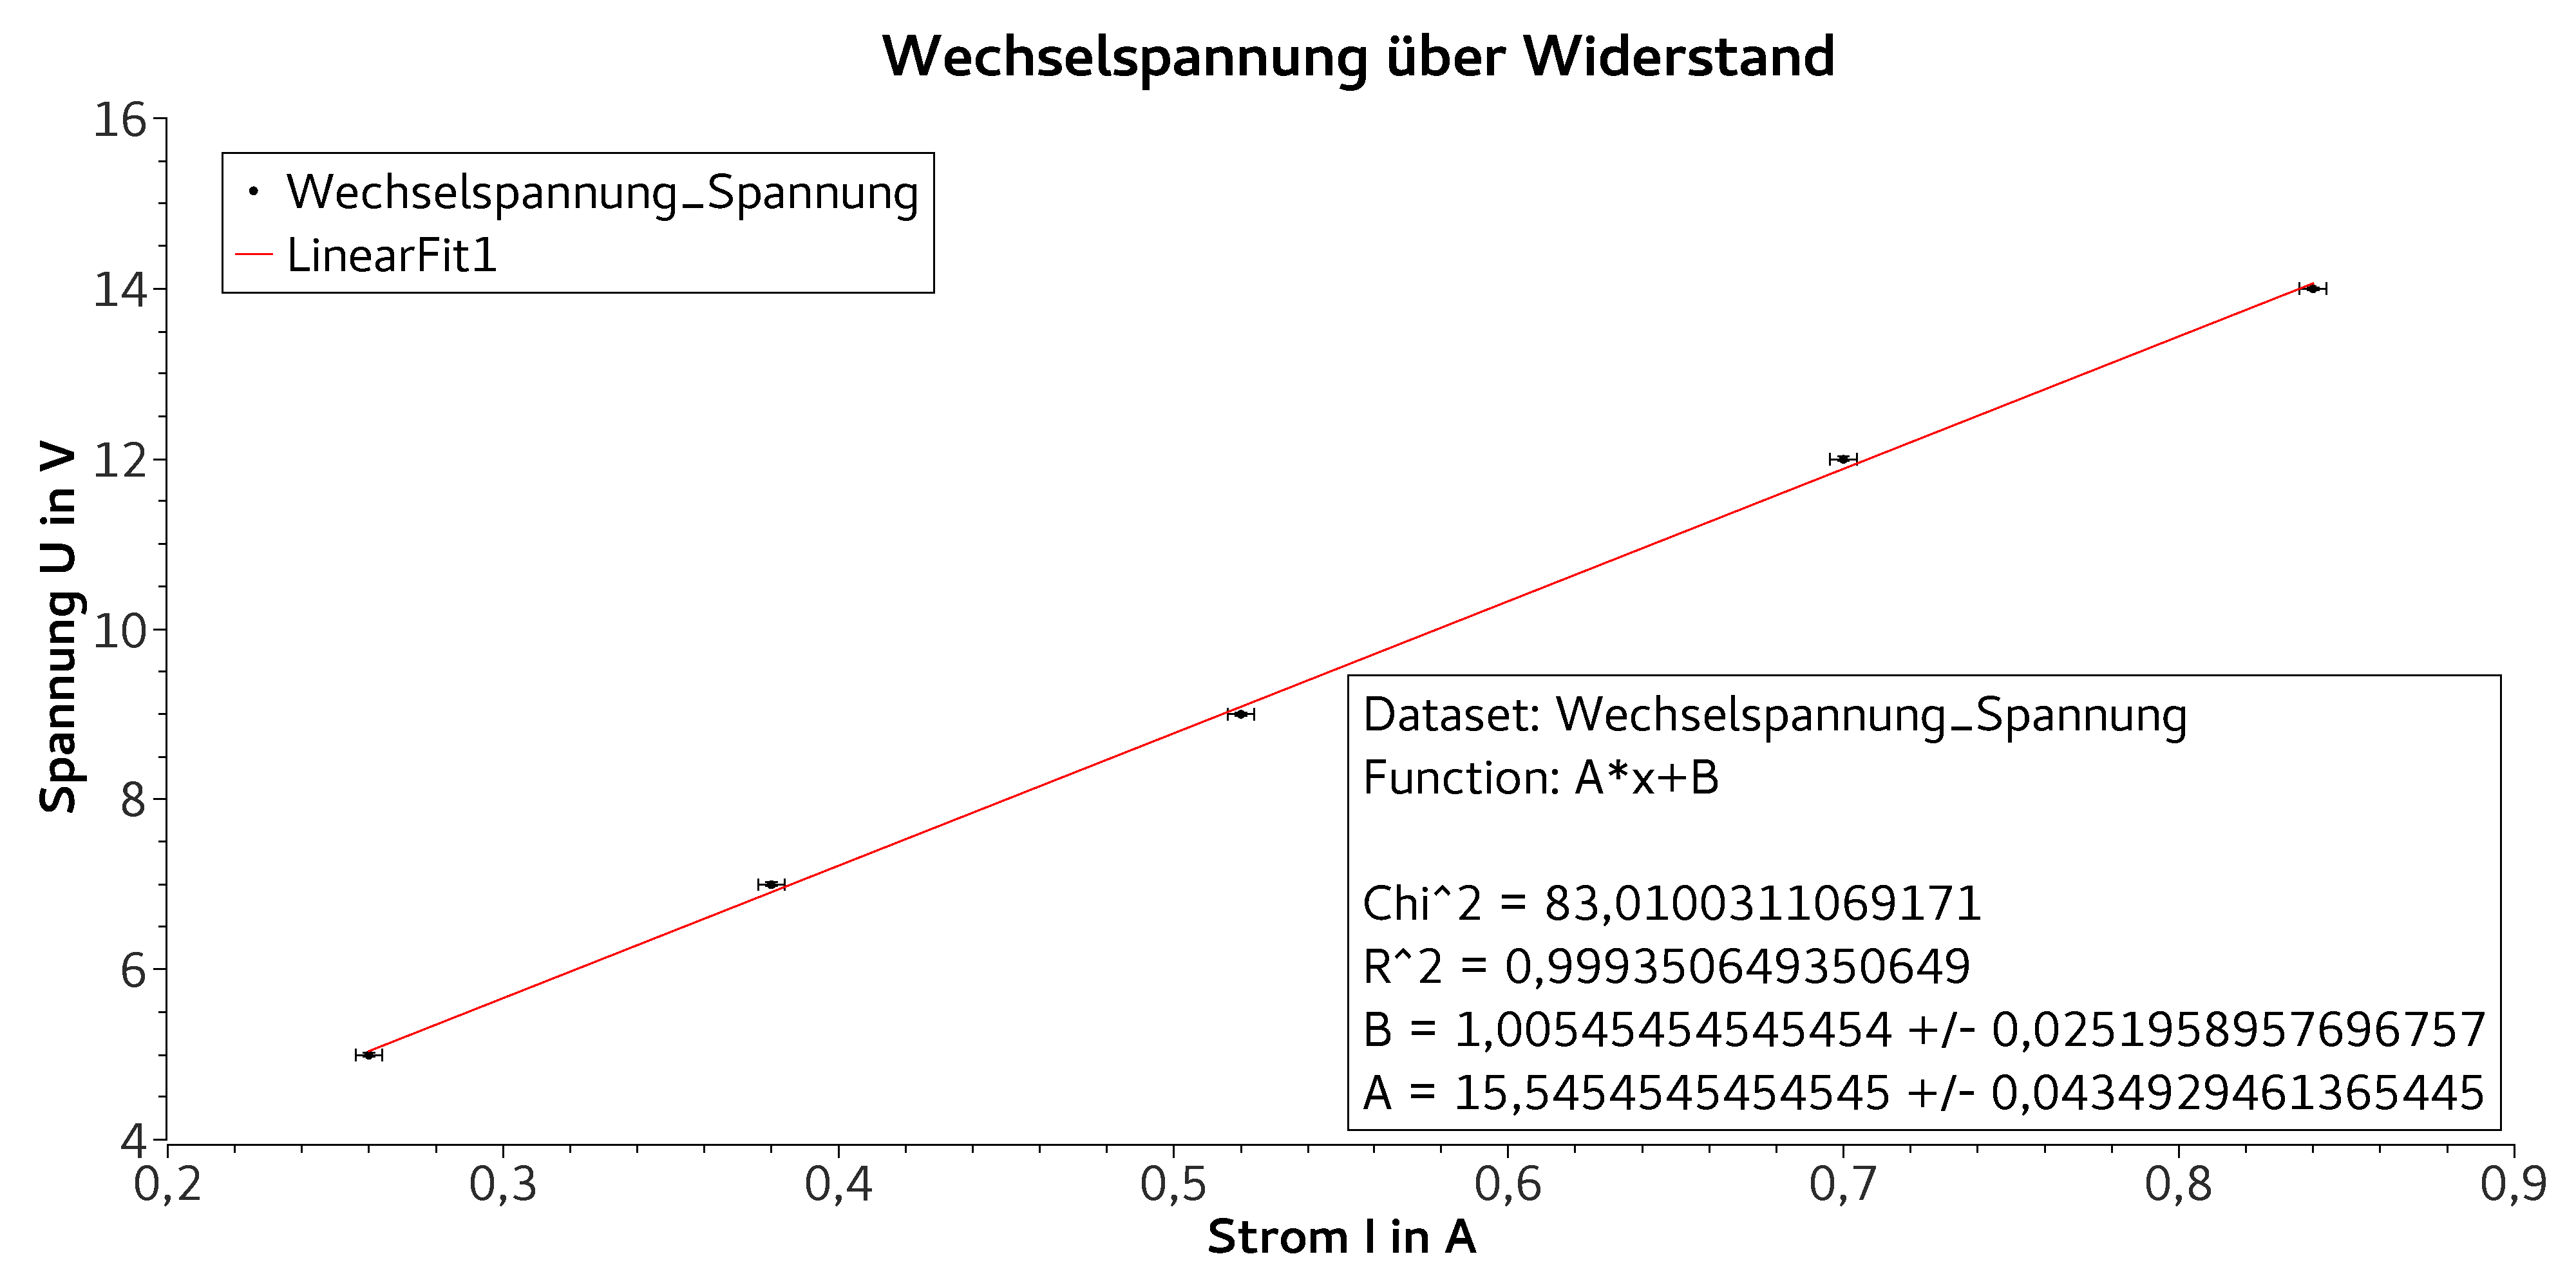
\includegraphics[width=1\textwidth]{WiderSpannungWechsel}
		\centering
		\caption{Die gemessene Spannung ist gegen den Strom aufgetragen.}
		\label{WiderSpannungWechsel}
		\centering
	\end{figure}
	\begin{figure}[tb]
		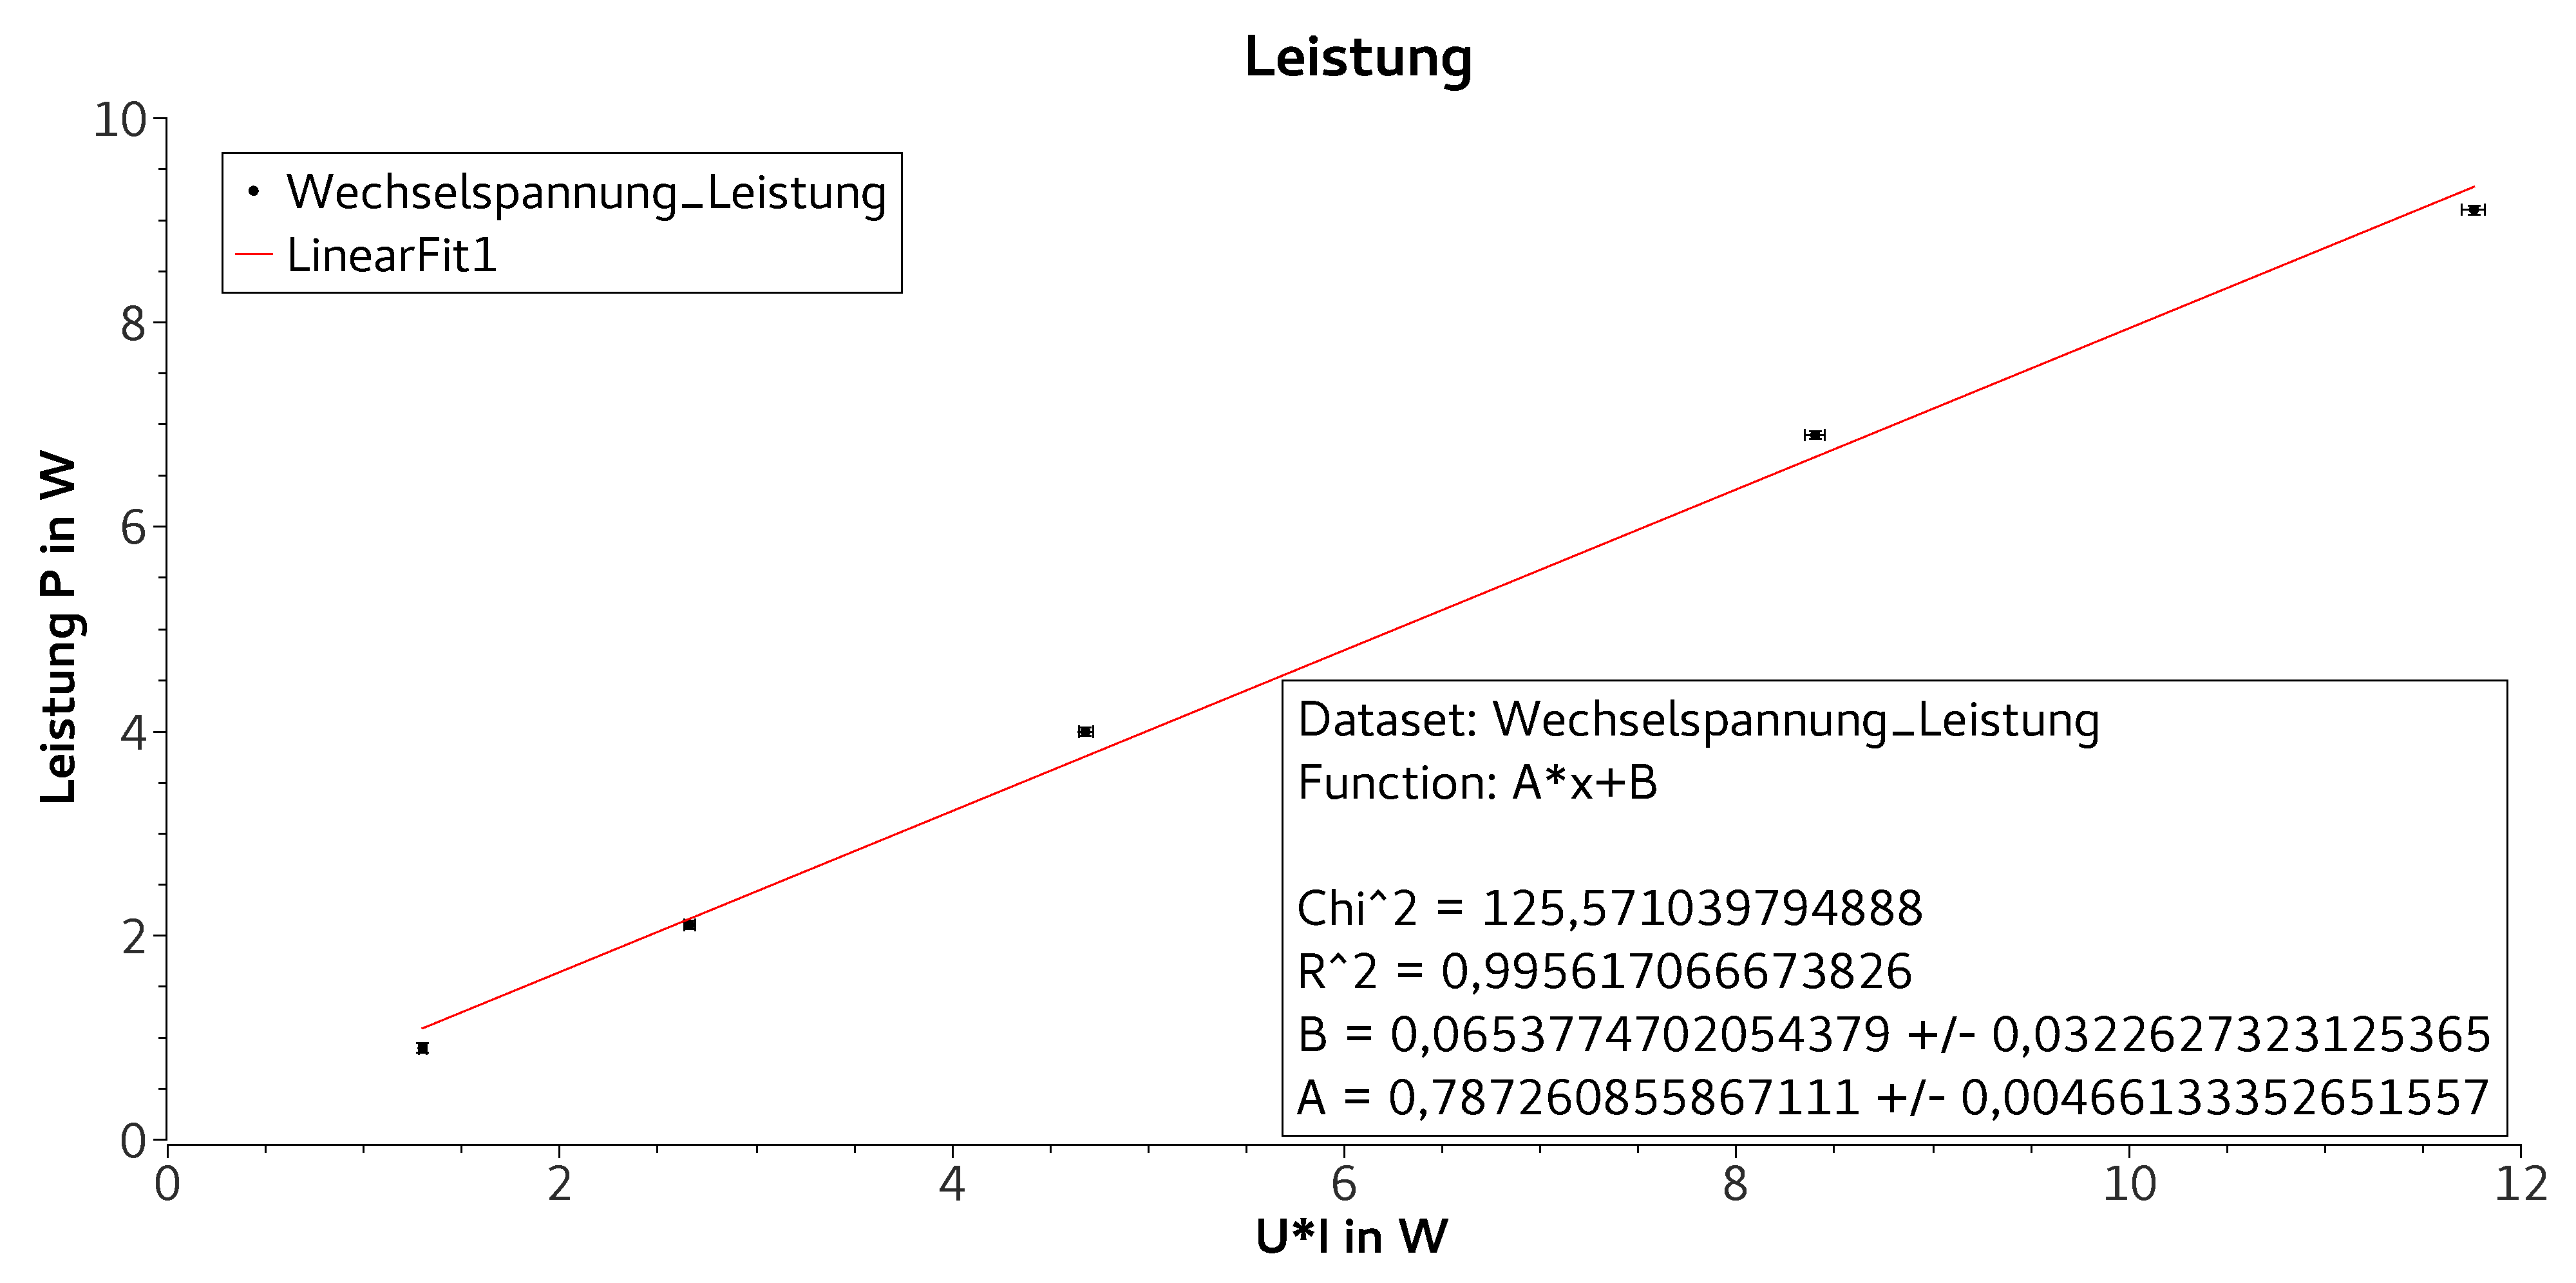
\includegraphics[width=1\textwidth]{WiderLeistungWechsel}
		\centering
		\caption{Die gemessene Leistung bei ist gegen das Produkt aus Strom und Spannung aufgetragen.}
		\label{WiderLeistungWechsel}
		\centering
	\end{figure}

	\begin{figure}[tb]
		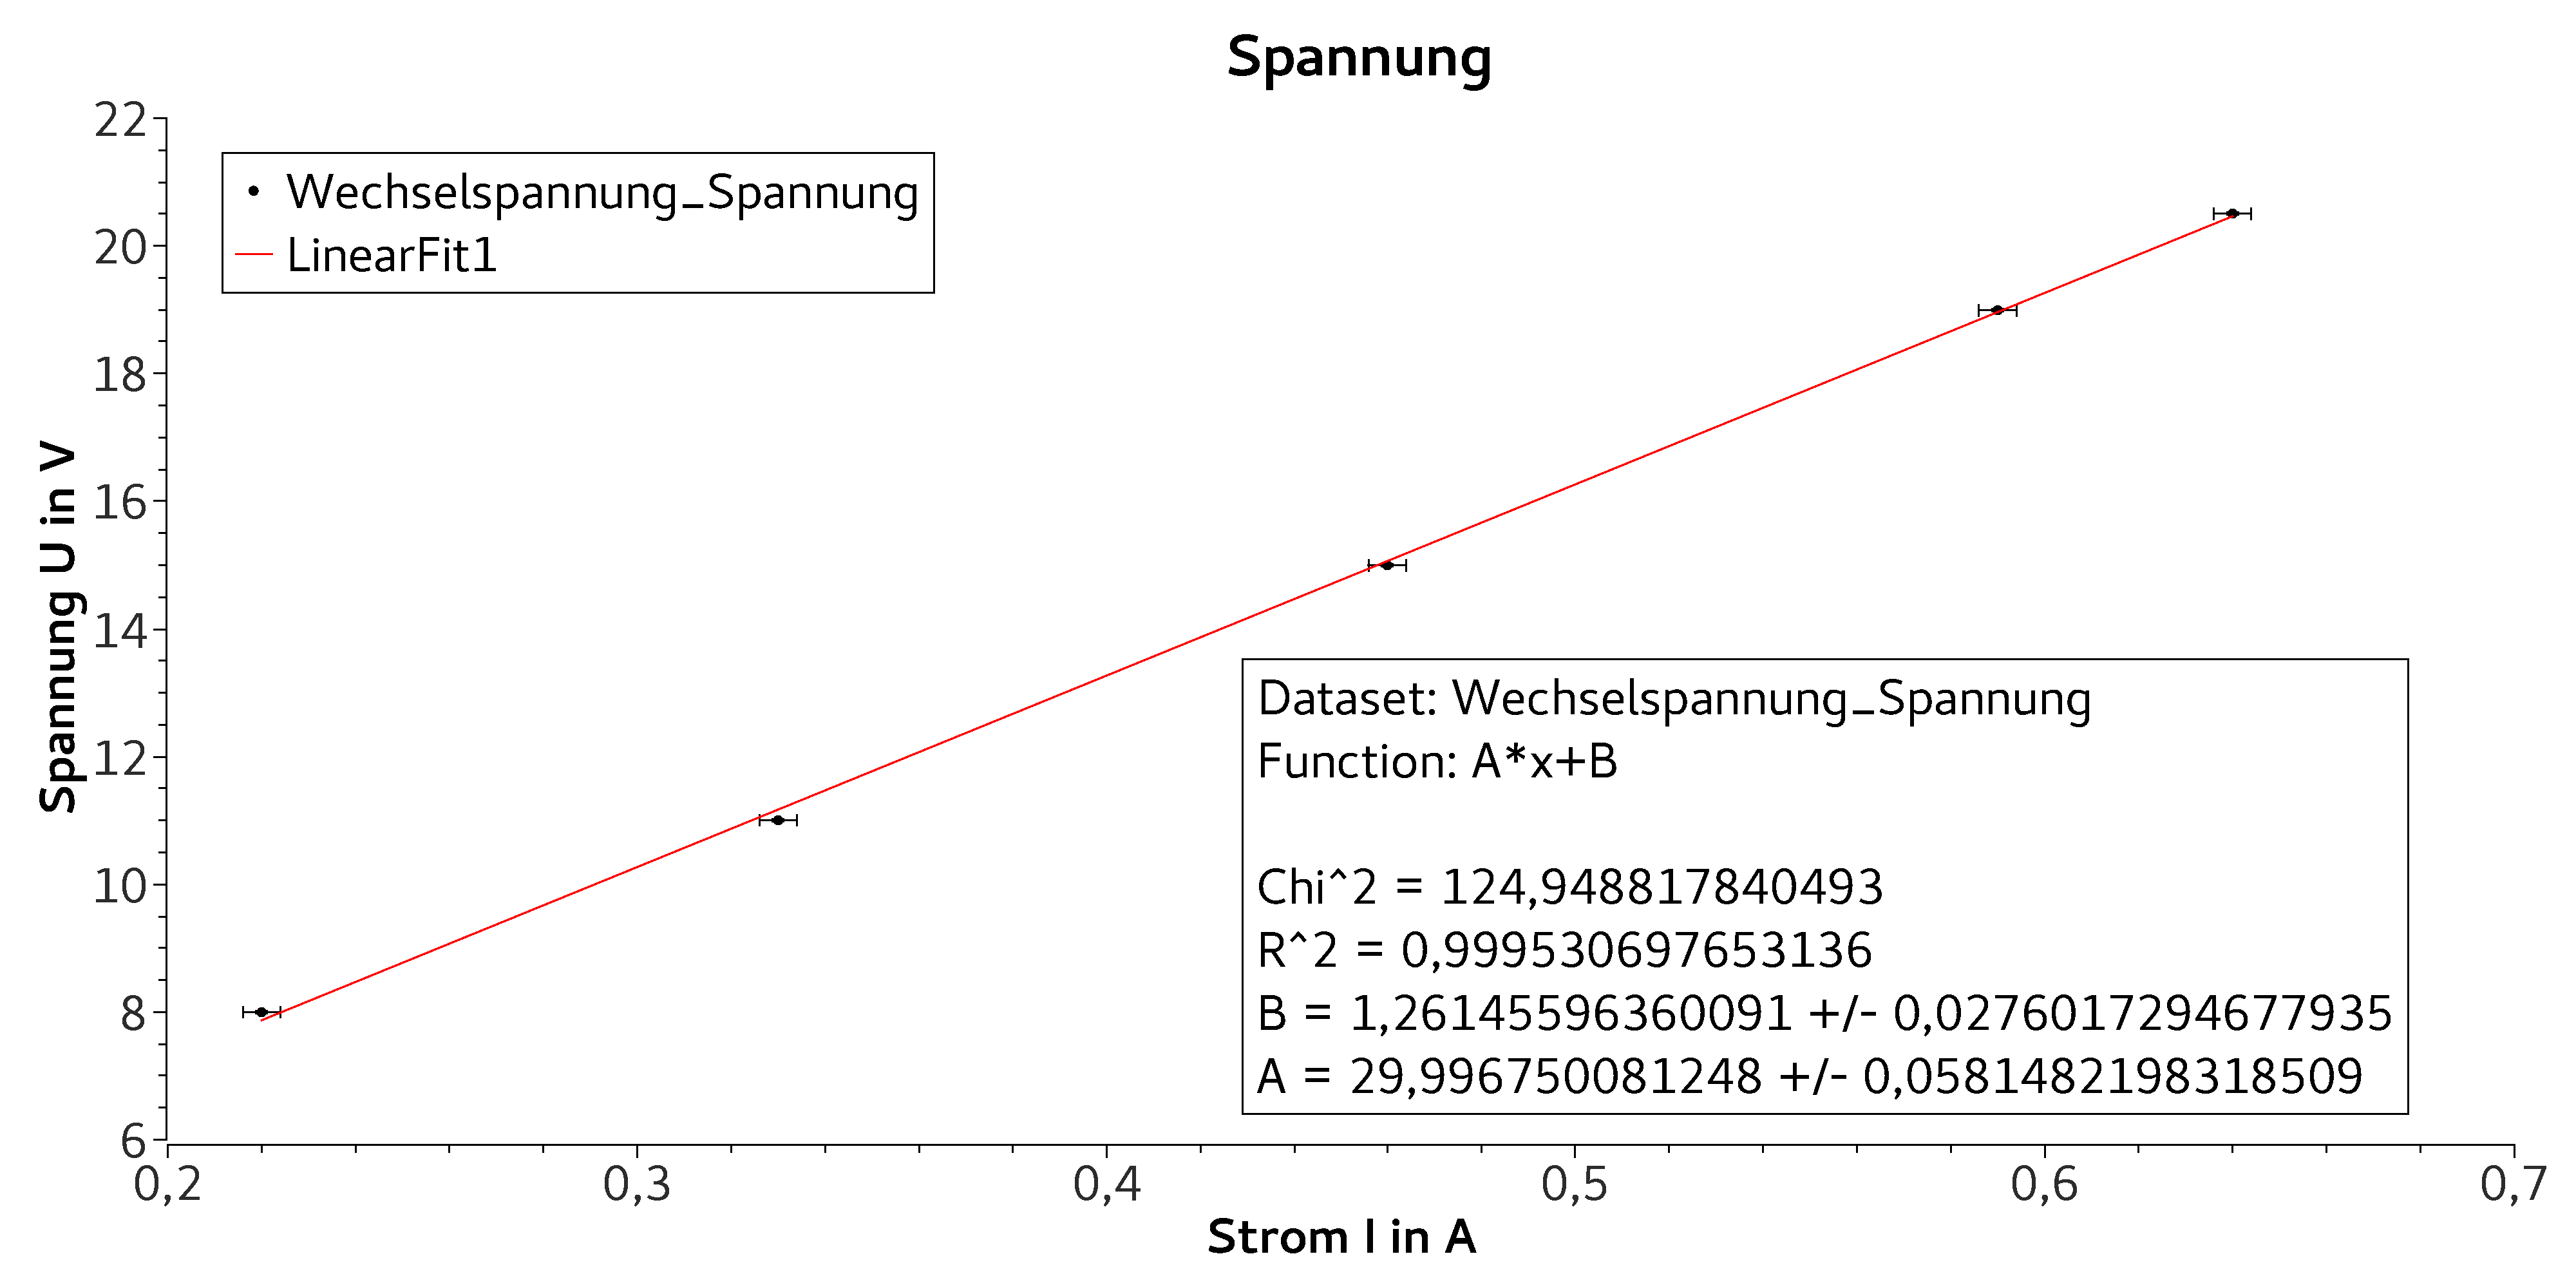
\includegraphics[width=1\textwidth]{SpuleSpannungWechsel}
		\centering
		\caption{Die gemessene Spannung bei ist gegen den Strom aufgetragen.}
		\label{SpuleSpannungWechsel}
		\centering
	\end{figure}
	\begin{figure}[tb]
		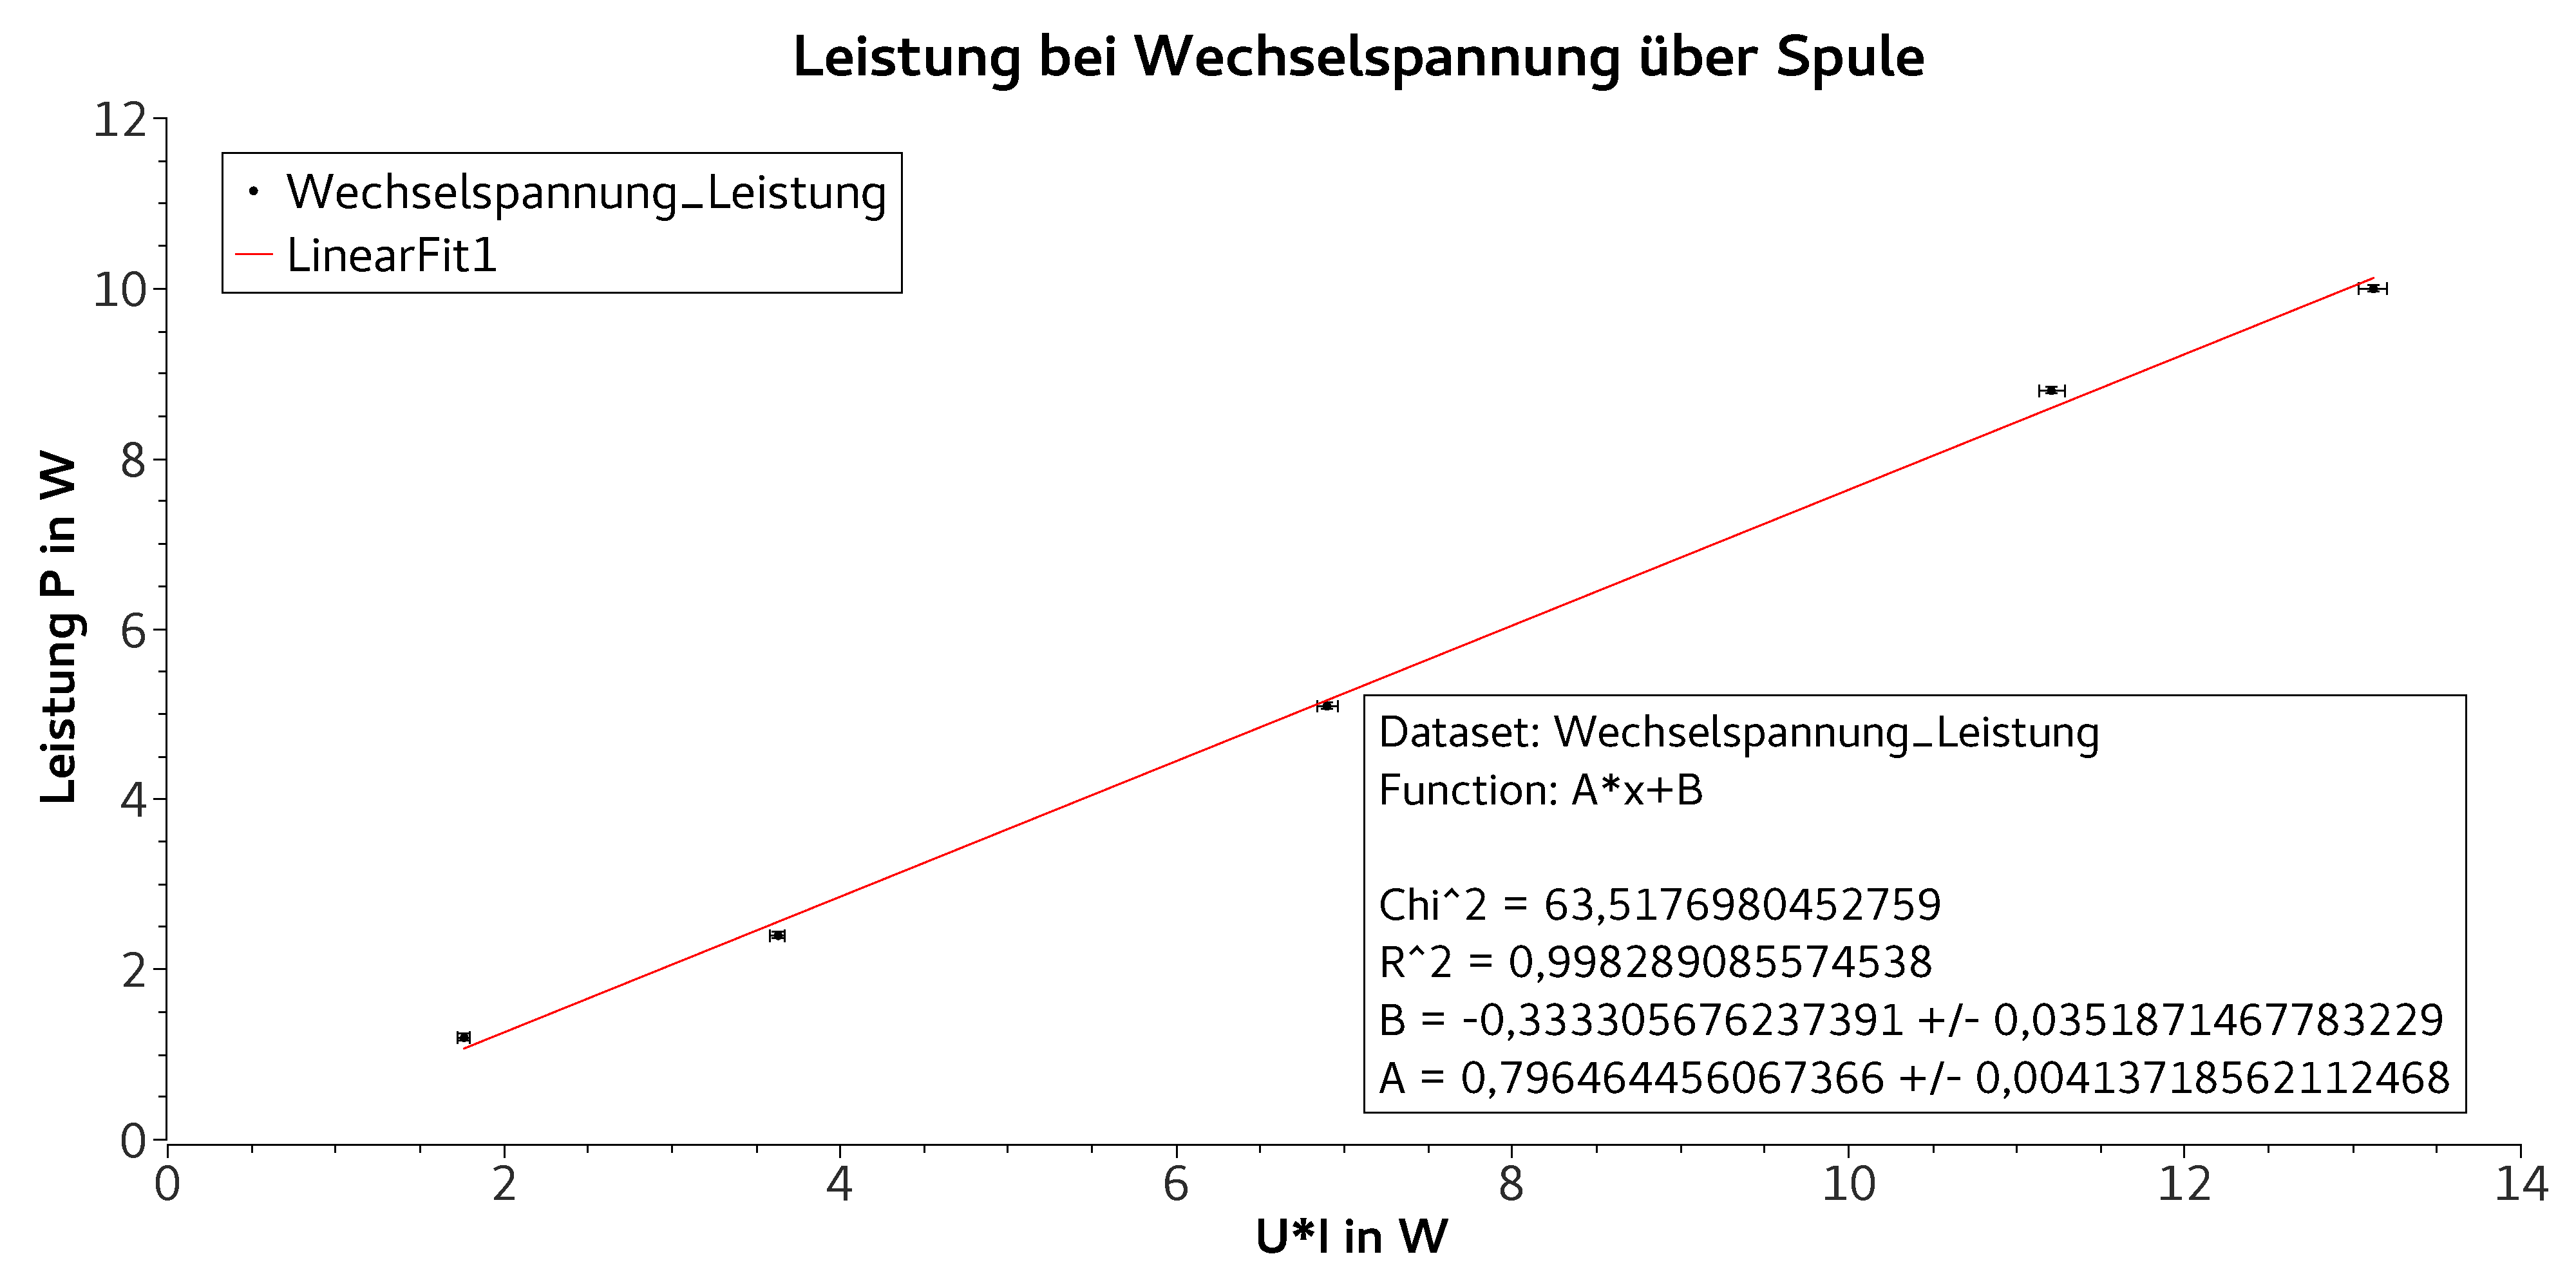
\includegraphics[width=1\textwidth]{SpuleLeistungWechsel}
		\centering
		\caption{Die gemessene Leistung bei ist gegen das Produkt aus Strom und Spannung aufgetragen.}
		\label{SpuleLeistungWechsel}
		\centering
	\end{figure}
	\begin{figure}[tb]
		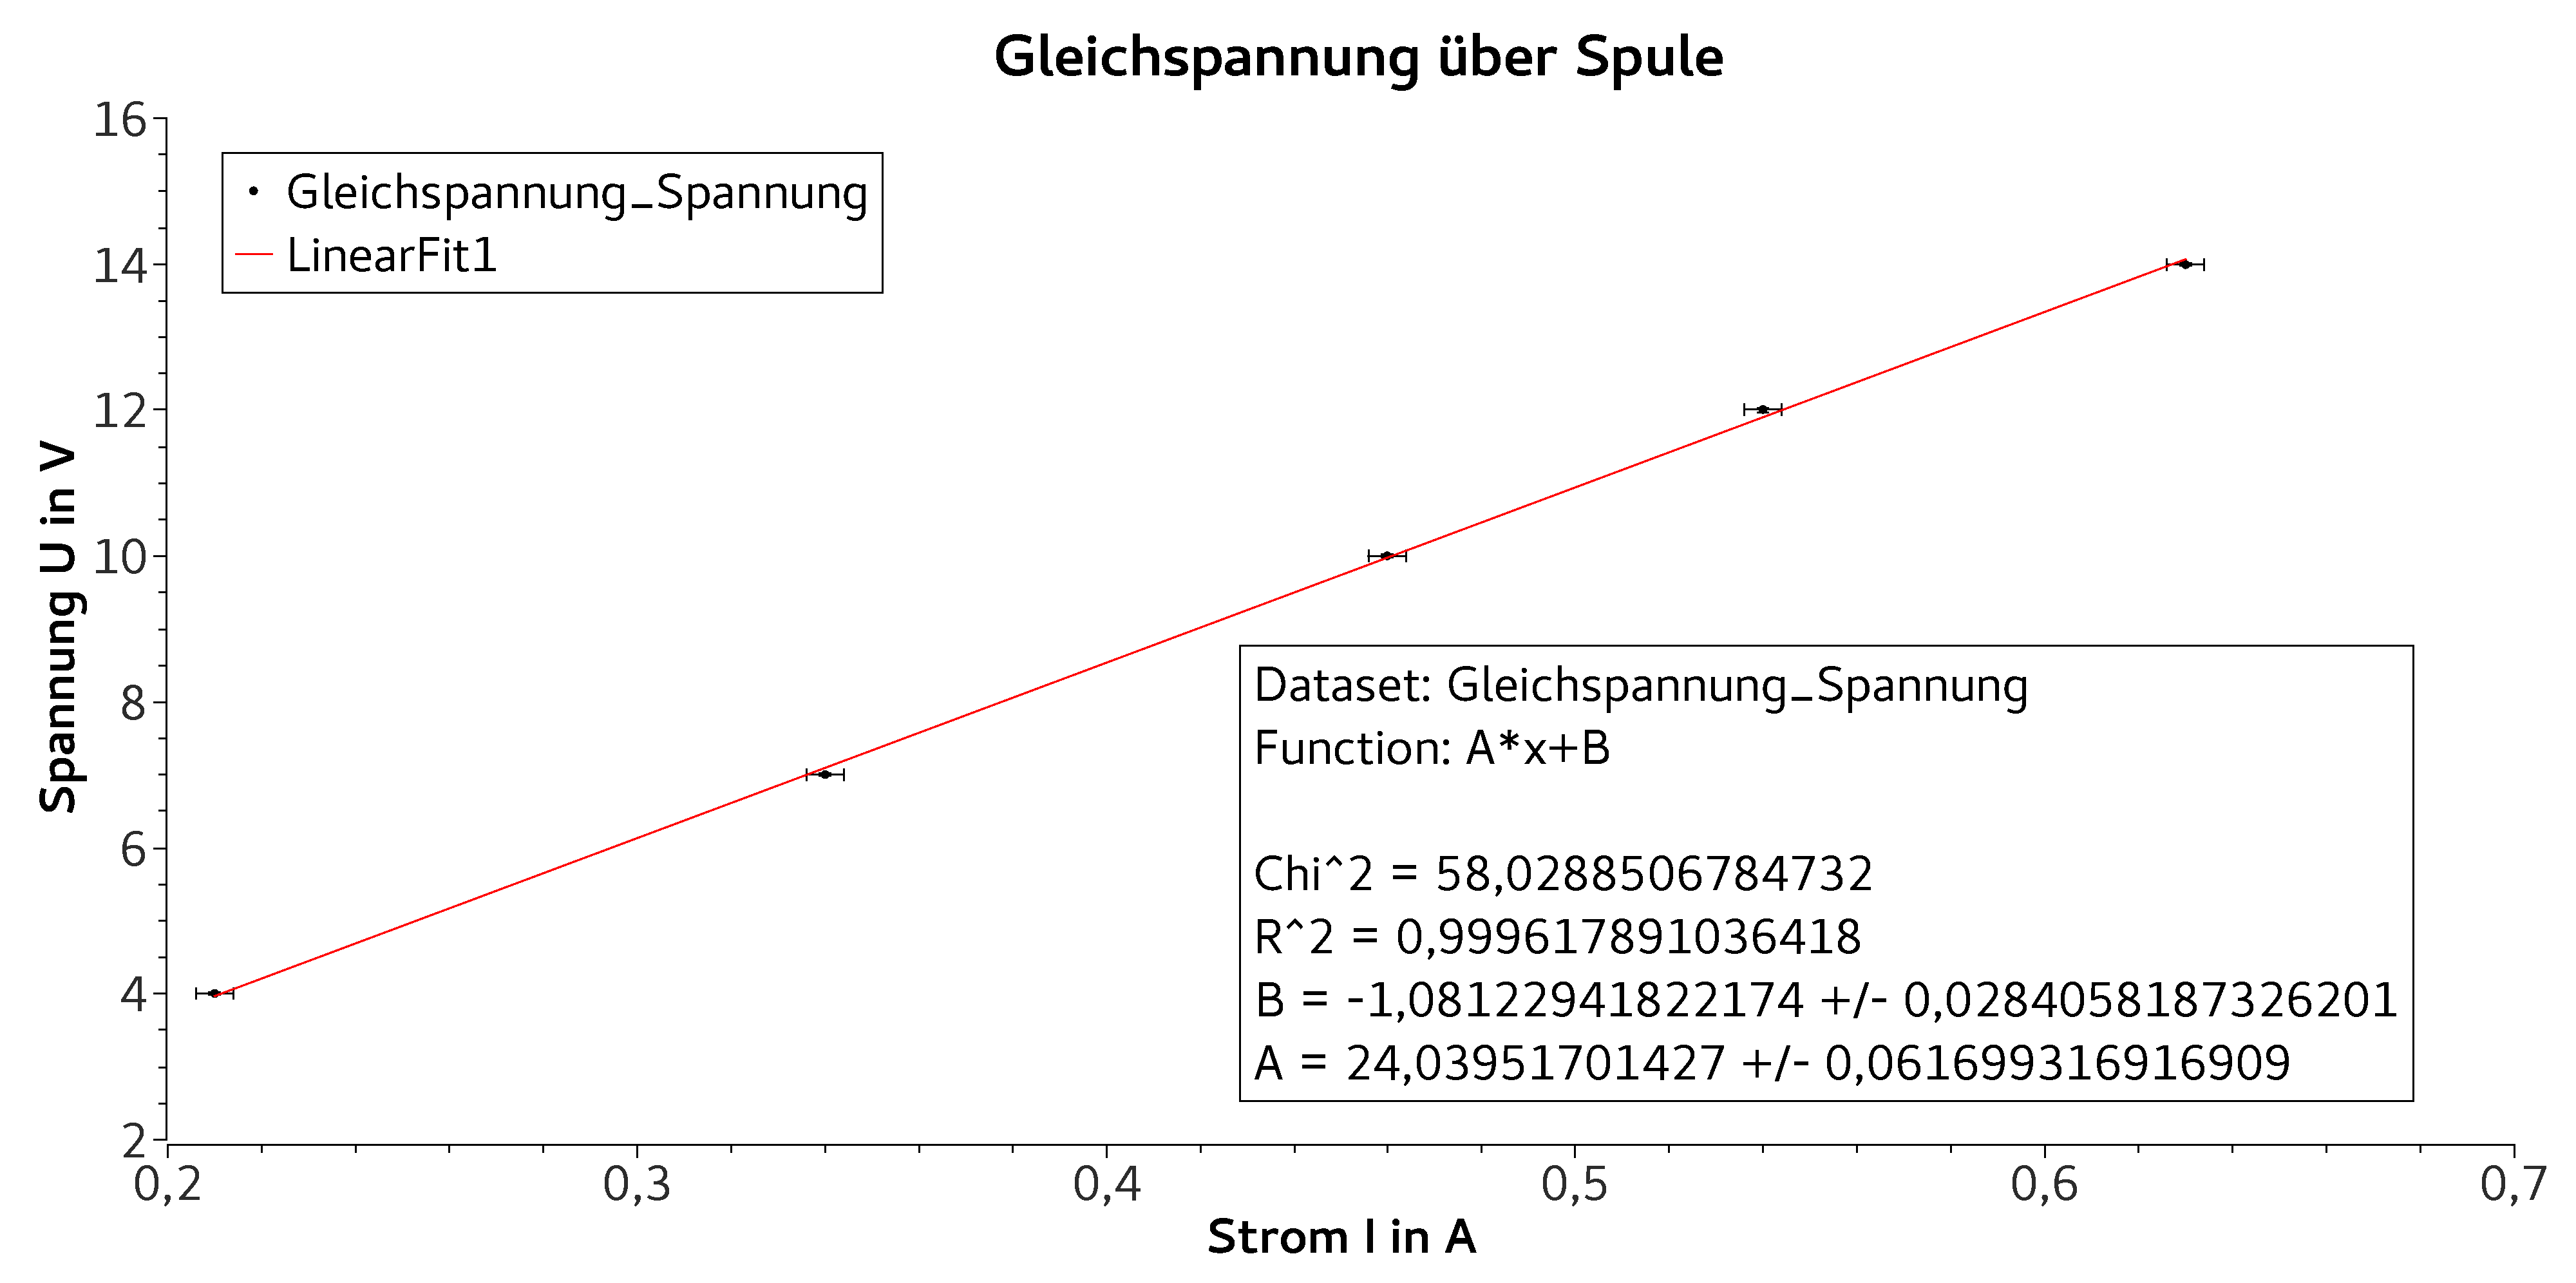
\includegraphics[width=1\textwidth]{SpuleSpannungGleich}
		\centering
		\caption{Die gemessene Spannung bei ist gegen den Strom aufgetragen.}
		\label{SpuleSpannungGleich}
		\centering
	\end{figure}
	
	\begin{figure}[tb]
		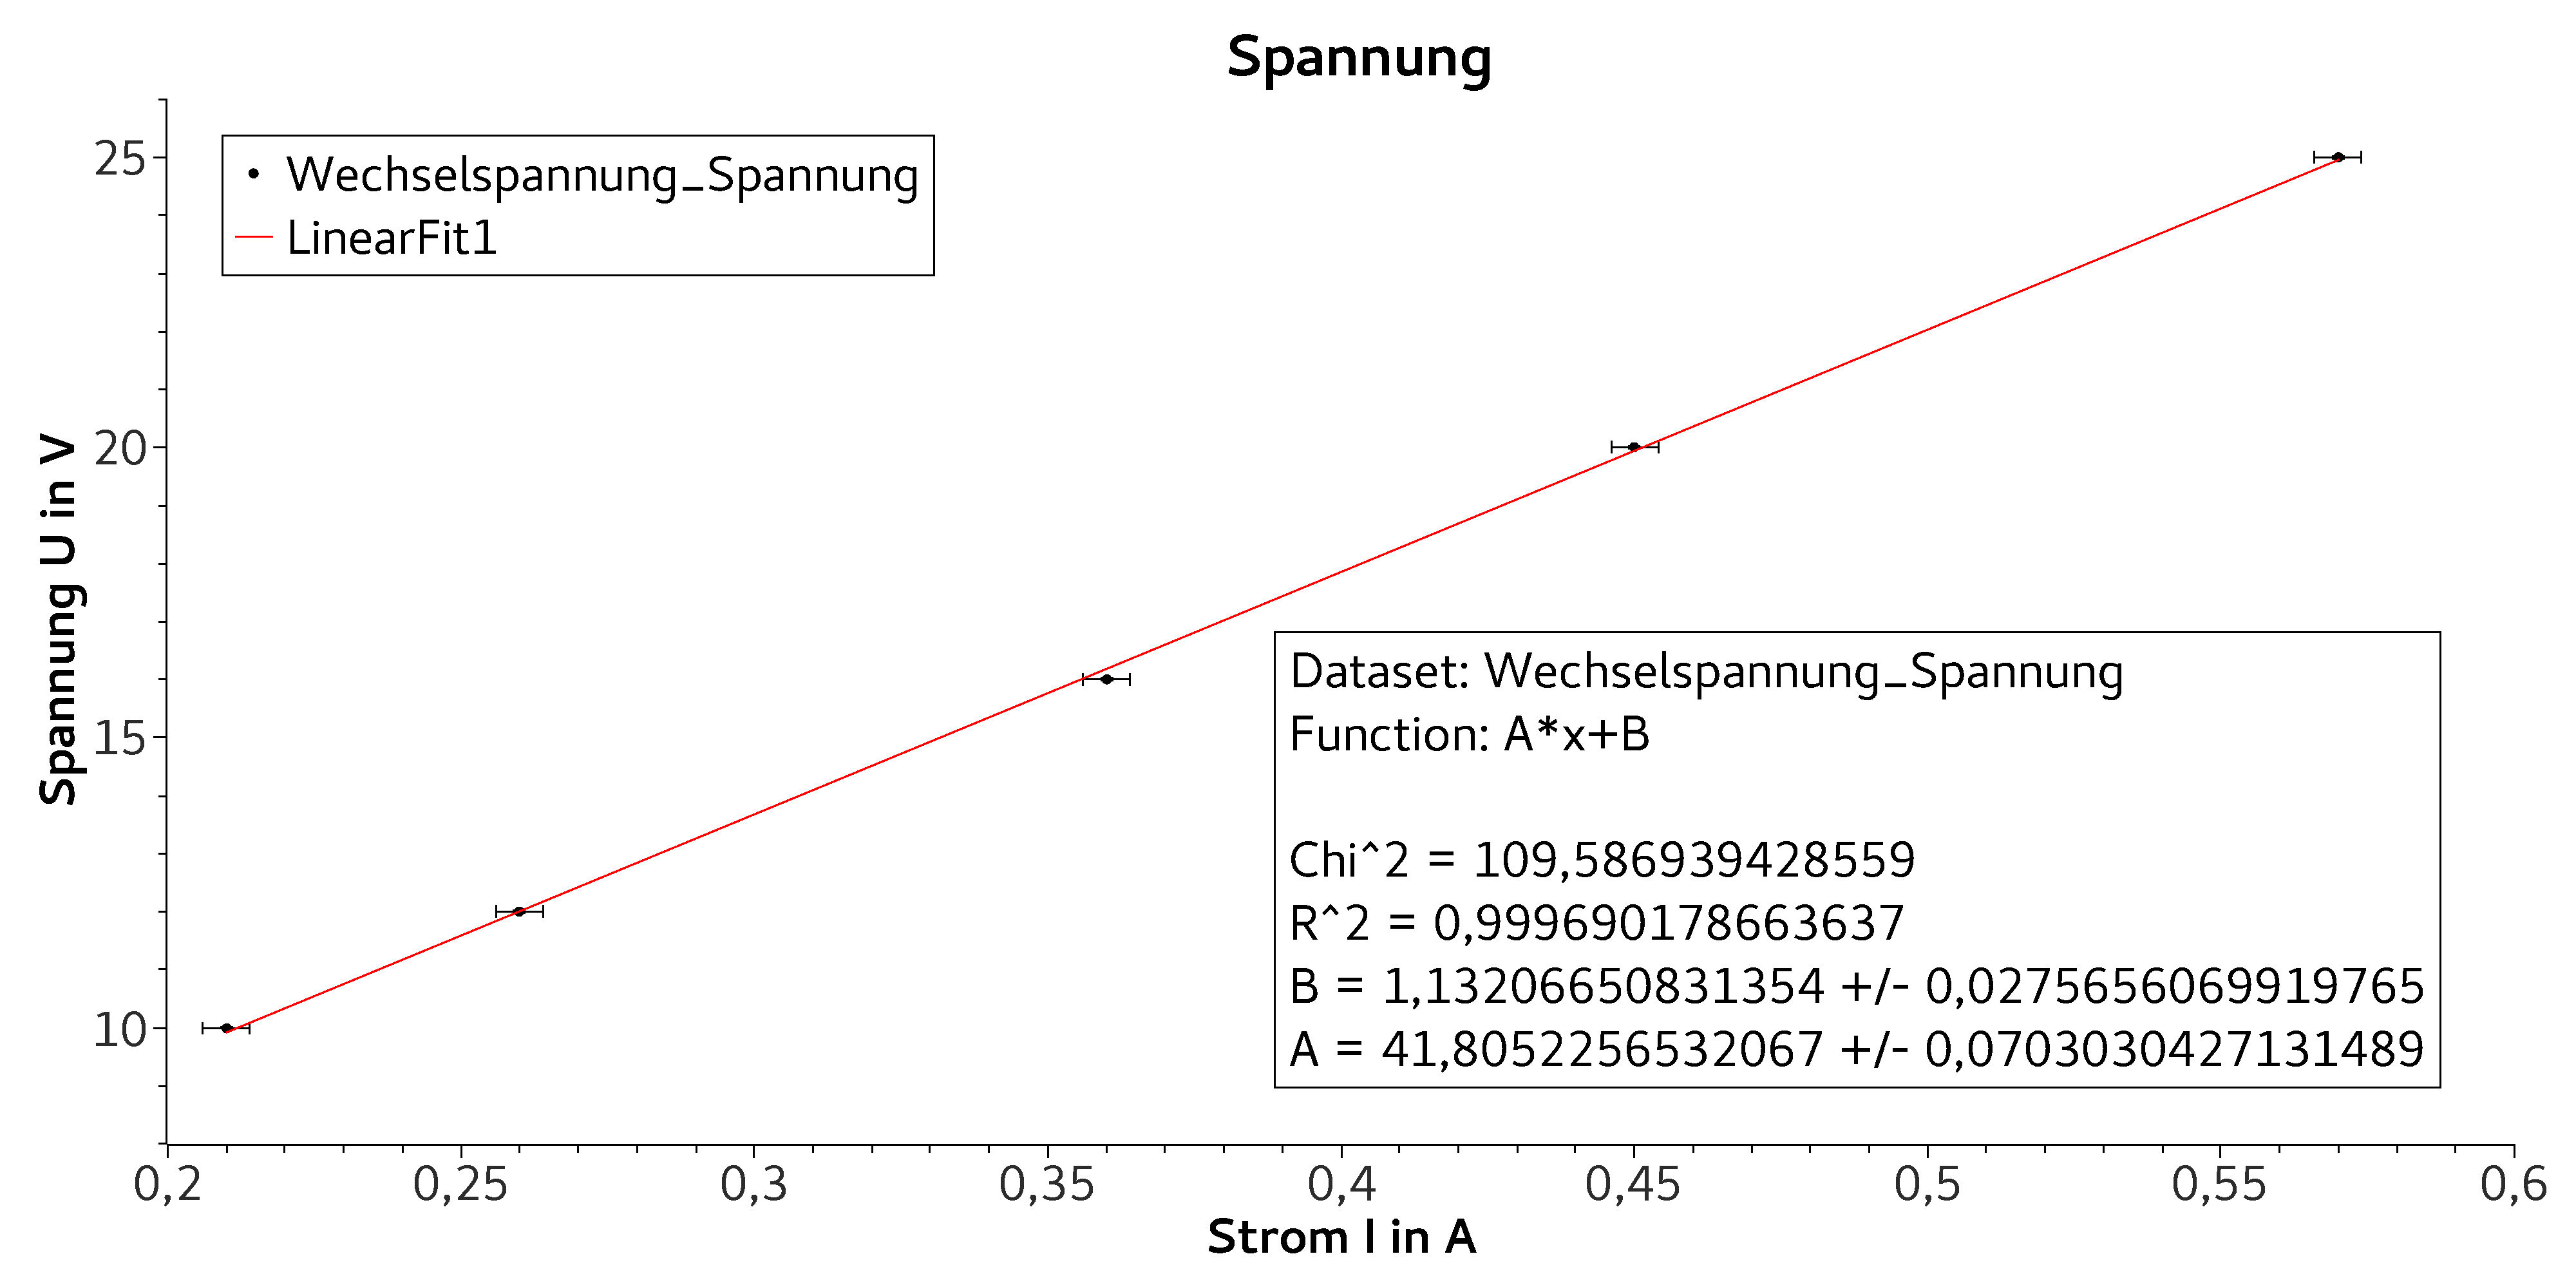
\includegraphics[width=1\textwidth]{KondensatorSpannungWechsel}
		\centering
		\caption{Die gemessene Spannung bei ist gegen den Strom aufgetragen.}
		\label{KondesatorSpannungWechsel}
		\centering
	\end{figure}
	\begin{figure}[tb]
		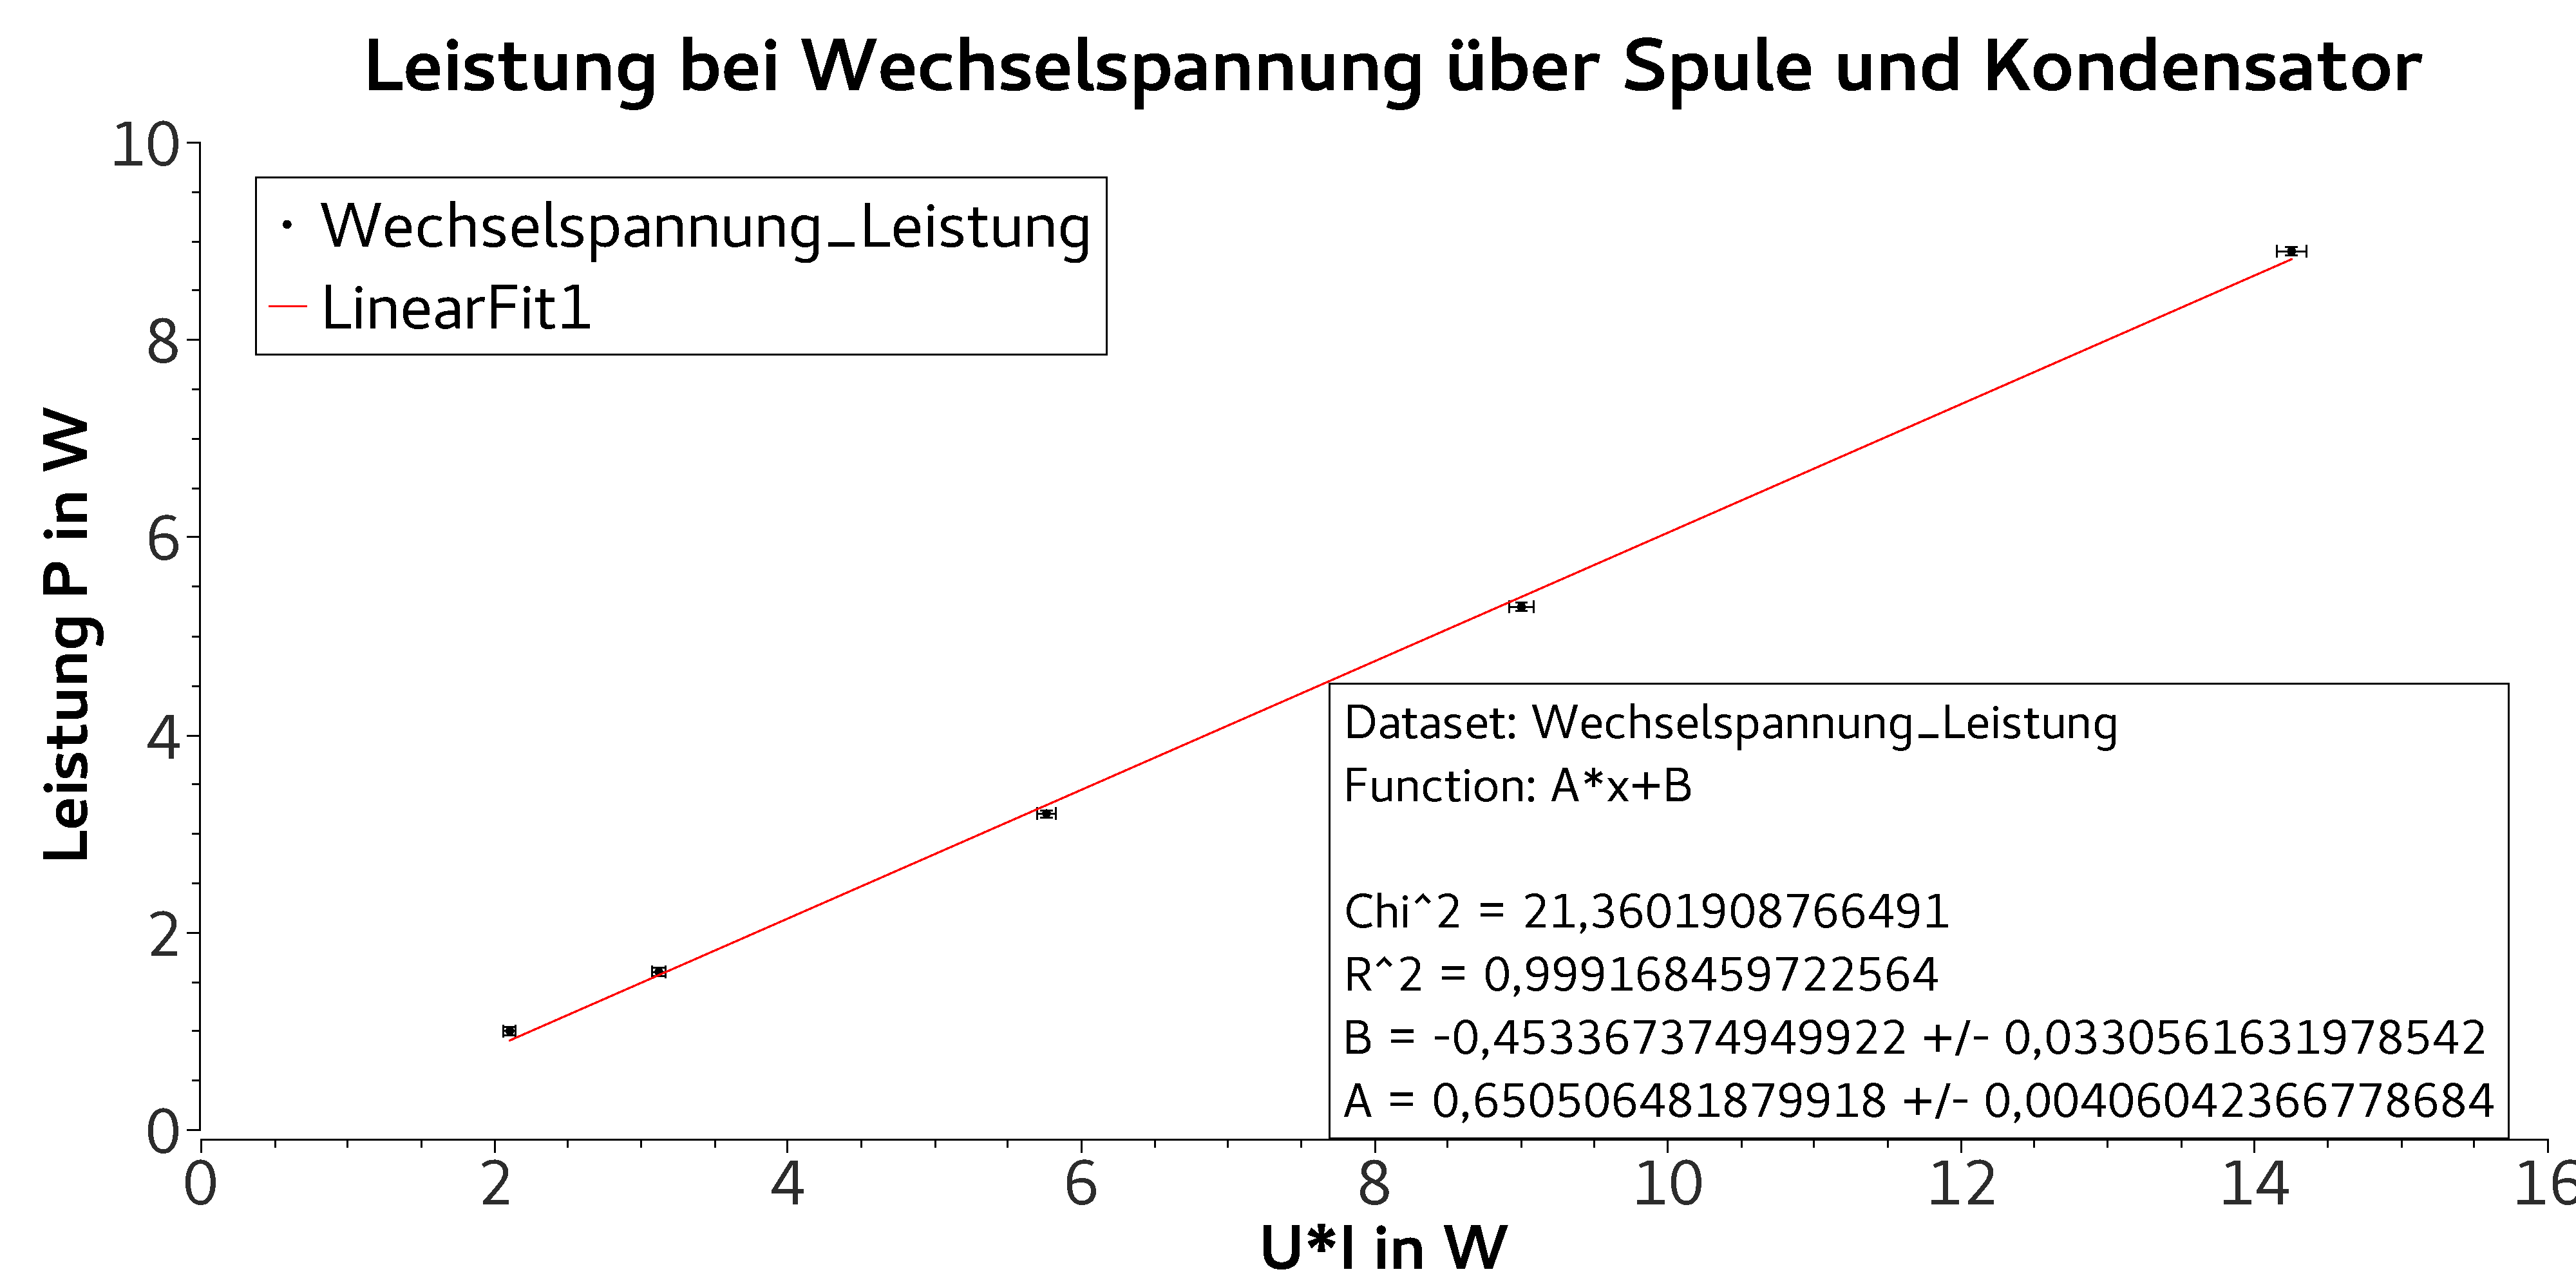
\includegraphics[width=1\textwidth]{KondensatorLeistungWechsel}
		\centering
		\caption{Die gemessene Leistung bei ist gegen das Produkt aus Strom und Spannung aufgetragen.}
		\label{KondesatorLeistungWechsel}
		\centering
	\end{figure}
	



	



	\subsection{Beobachtung}

	\subsection{Diskussion}
	%TODO Bezug/Nutzten oder sonst was
	%TODO auch hier die Hypothese wiederholen
	
	\section{Schlussfolgerung}
	%TODO Rückgriff auf Hypothese und drittes Nennen dieser
	
	%TODO Quellen zitieren, Websiten mit Zugriffsdatum
	%TODO Verweise auf das Laborbuch (sind erlaubt)
	%TODO Tabelle + Bilder mit Beschriftung
	%\printbibliography
\end{document}
